\documentclass[a4paper, 12pt]{book}

% Paquetes básicos de LATEX
\usepackage{amsmath, amssymb}
\usepackage[T1]{fontenc}
\usepackage[utf8]{inputenc}
\usepackage[spanish]{babel}

% Título y autor
\title{Título del proyecto}
\author{Daniel Gómez}

% Para cambiar márgenes
\usepackage[a4paper]{geometry}
\geometry{left=3cm, right=3cm}

% Para quitar encabezado, pie de página y numeración en páginas vacías
\usepackage{emptypage}

% Para añadir figuras y su path
\usepackage{graphicx}
\graphicspath{{figures/}}

% Para modificar encabezados y pie de página
\usepackage{fancyhdr}
\fancyhf{} % Limpia los encabezados y pie de página
\lhead[\leftmark]{Daniel G. R.}
\rhead[Daniel G. R.]{\rightmark}
\cfoot[\thepage]{\thepage}

% Añadir línea separatoria en el encabezado
\renewcommand{\headrulewidth}{0.4pt}

% Paquete para añadir enlaces entre referencias
\usepackage[hidelinks]{hyperref}

% Comando creado para añadir figuras más rápido y más limpio
\newcommand{\addimage}[4]{
\begin{figure}[h]
\begin{center} \label{fig:#2}
\includegraphics[width=#4\textwidth]{#1}
\end{center}
\caption{#3}
\end{figure}
}



% Paquete para bibliografías
\usepackage[
backend=biber,
style=numeric,
sorting=none,
dateabbrev=false,
citestyle=numeric
]{biblatex}

\addbibresource{bibliografia.bib}

\widowpenalty=10000
\clubpenalty=10000

\usepackage[font=footnotesize, skip=4pt, justification=centering]{caption}

\raggedbottom

\usepackage{array}

\begin{document}


\pagestyle{fancy}

\maketitle

\chapter*{Resumen}
\addcontentsline{toc}{chapter}{Resumen}
\pagenumbering{Roman}
\setcounter{page}{5} % Habrá que modificarlo cuando se añadan el resto de páginas

En la actualidad, los robots móviles utilizan mapas para localizarse. Estos mapas son generados a partir de los barridos de un láser, que detecta los objetos y sus distancias, obteniendo zonas ocupadas y desocupadas. Sin embargo, existen elementos en el entorno que no pertenecen a la estructura del mismo y pueden variar su posición de un día para otro, invalidando el mapa generado. El objetivo de este trabajo es aprovechar la información de profundidad proporcionada por sensores RGBD para generar un mapa donde únicamente se representen los elementos estructurales. Para ello se han procesado los datos de profundidad y se han guardado los elementos que estén más alejados, eliminando los objetos que se encuentren frente a una pared. Paralelamente, se ha utilizado la imagen de color de la cámara para realizar un proceso de detección de objetos mediante una red neuronal convolucional ya entrenada, para realizar un posterior análisis de fiabilidad de la red. Los resultados obtenidos son algo difusos y no permiten la aplicación de esta metodología al mundo real. Sin embargo se atisba que, puliendo algunos aspectos hallados durante el transcurso del trabajo, se puede conseguir un buen producto final.\\




\chapter*{Abstract}
\addcontentsline{toc}{chapter}{Abstract}

\chapter*{Agradecimientos}
\addcontentsline{toc}{chapter}{Agradecimientos}

Quisiera transmitir mi más sincero agradecimiento a todos los que han ayudado a cerrar esta etapa tan bonita.\\

Gracias a mis tutores Javier González Monroy y Cipriano Galindo Andrades por brindarme la oportunidad de realizar este trabajo. Gracias por ayudarme en todas las etapas y por hacerlo siempre con tanta amabilidad.\\

Gracias a mis padres, Manolo y Rosa, y a mi hermano Manuel por apoyarme en los momentos más difíles durante estos cuatro años.\\

Gracias a mi pareja, Laura, por ese apoyo incondicional y por escuchar mis males y quejas sin poner ni tan siquiera alguna mala cara.\\

A todos ellos, muchas gracias.\\

\tableofcontents

\cleardoublepage
\addcontentsline{toc}{chapter}{Lista de figuras} % para que aparezca en el indice de contenidos
\listoffigures % indice de figuras

\cleardoublepage
\addcontentsline{toc}{chapter}{Lista de tablas} % para que aparezca en el indice de contenidos
\listoftables % indice de tablas

\part{Introducción}
\pagenumbering{arabic}

\chapter{Introducción y visión general}


En este capítulo se hará una breve introducción para entender el contexto de este trabajo y el porqué de la necesidad del mismo. Se comentará la importancia de la localización para los seres humanos y se hará una introducción sobre los mapas utilizados por los robots para localizarse. Finalmente se expondrá la estructura del documento.\\

\section{La localización como una necesidad}

Que levante la mano quien no se ha perdido alguna vez por los despachos de alguna de las facultades, sobre todo en esos ambientes prácticamente idénticos entre sí. Todo ser humano alguna vez se ha parado en seco, ha mirado a un lado y a otro con cara de desaprobación y se ha preguntado: \textit{¿dónde estoy?} Estas situaciones, a veces incómodas, se deben esencialmente a que todo ser vivo con capacidad para desplazarse por un entorno necesita localizarse y orientarse si quiere alcanzar un objetivo, más aún si dicho entorno es totalmente desconocido.\\

A lo largo de los años, los seres humanos hemos utilizado multitud de métodos para la orientación, incluso en las situaciones más desfavorables. Un estudio para la revista \textit{The Royal Society} de la Universidad de Rennes sostiene que los vikingos usaban una variedad de calcita para calcular dónde se encontraba el sol utilizando la polarización de la luz dispersada por las nubes. Esta piedra solar se llama ``Espato de Islandia'' y les permitía orientarse incluso en fechas donde el sol parecía no querer mostrarse, algo que sucede muy frecuentemente en los mares nórdicos \cite{vikingos}. Hoy en día, con el uso de la tecnología GPS y de aplicaciones que la implementan como Google Maps, hemos cambiado esa piedra solar por un dispositivo electrónico que, no solo nos localiza y orienta en prácticamente cualquier situación, sino que lo hace con un error casi despreciable. Pese al avance de las tecnología de localización como GPS, existen ciertas situaciones en las que es complicado aprovecharse de ellas, como por ejemplo en los entornos indoor. En estos caso, los satélites no son capaces de comunicarse con nuestros dispositivos, por lo que necesitamos otro mecanismo para localizarnos.\\

%\begin{figure}[H]
%	\begin{center} 
%	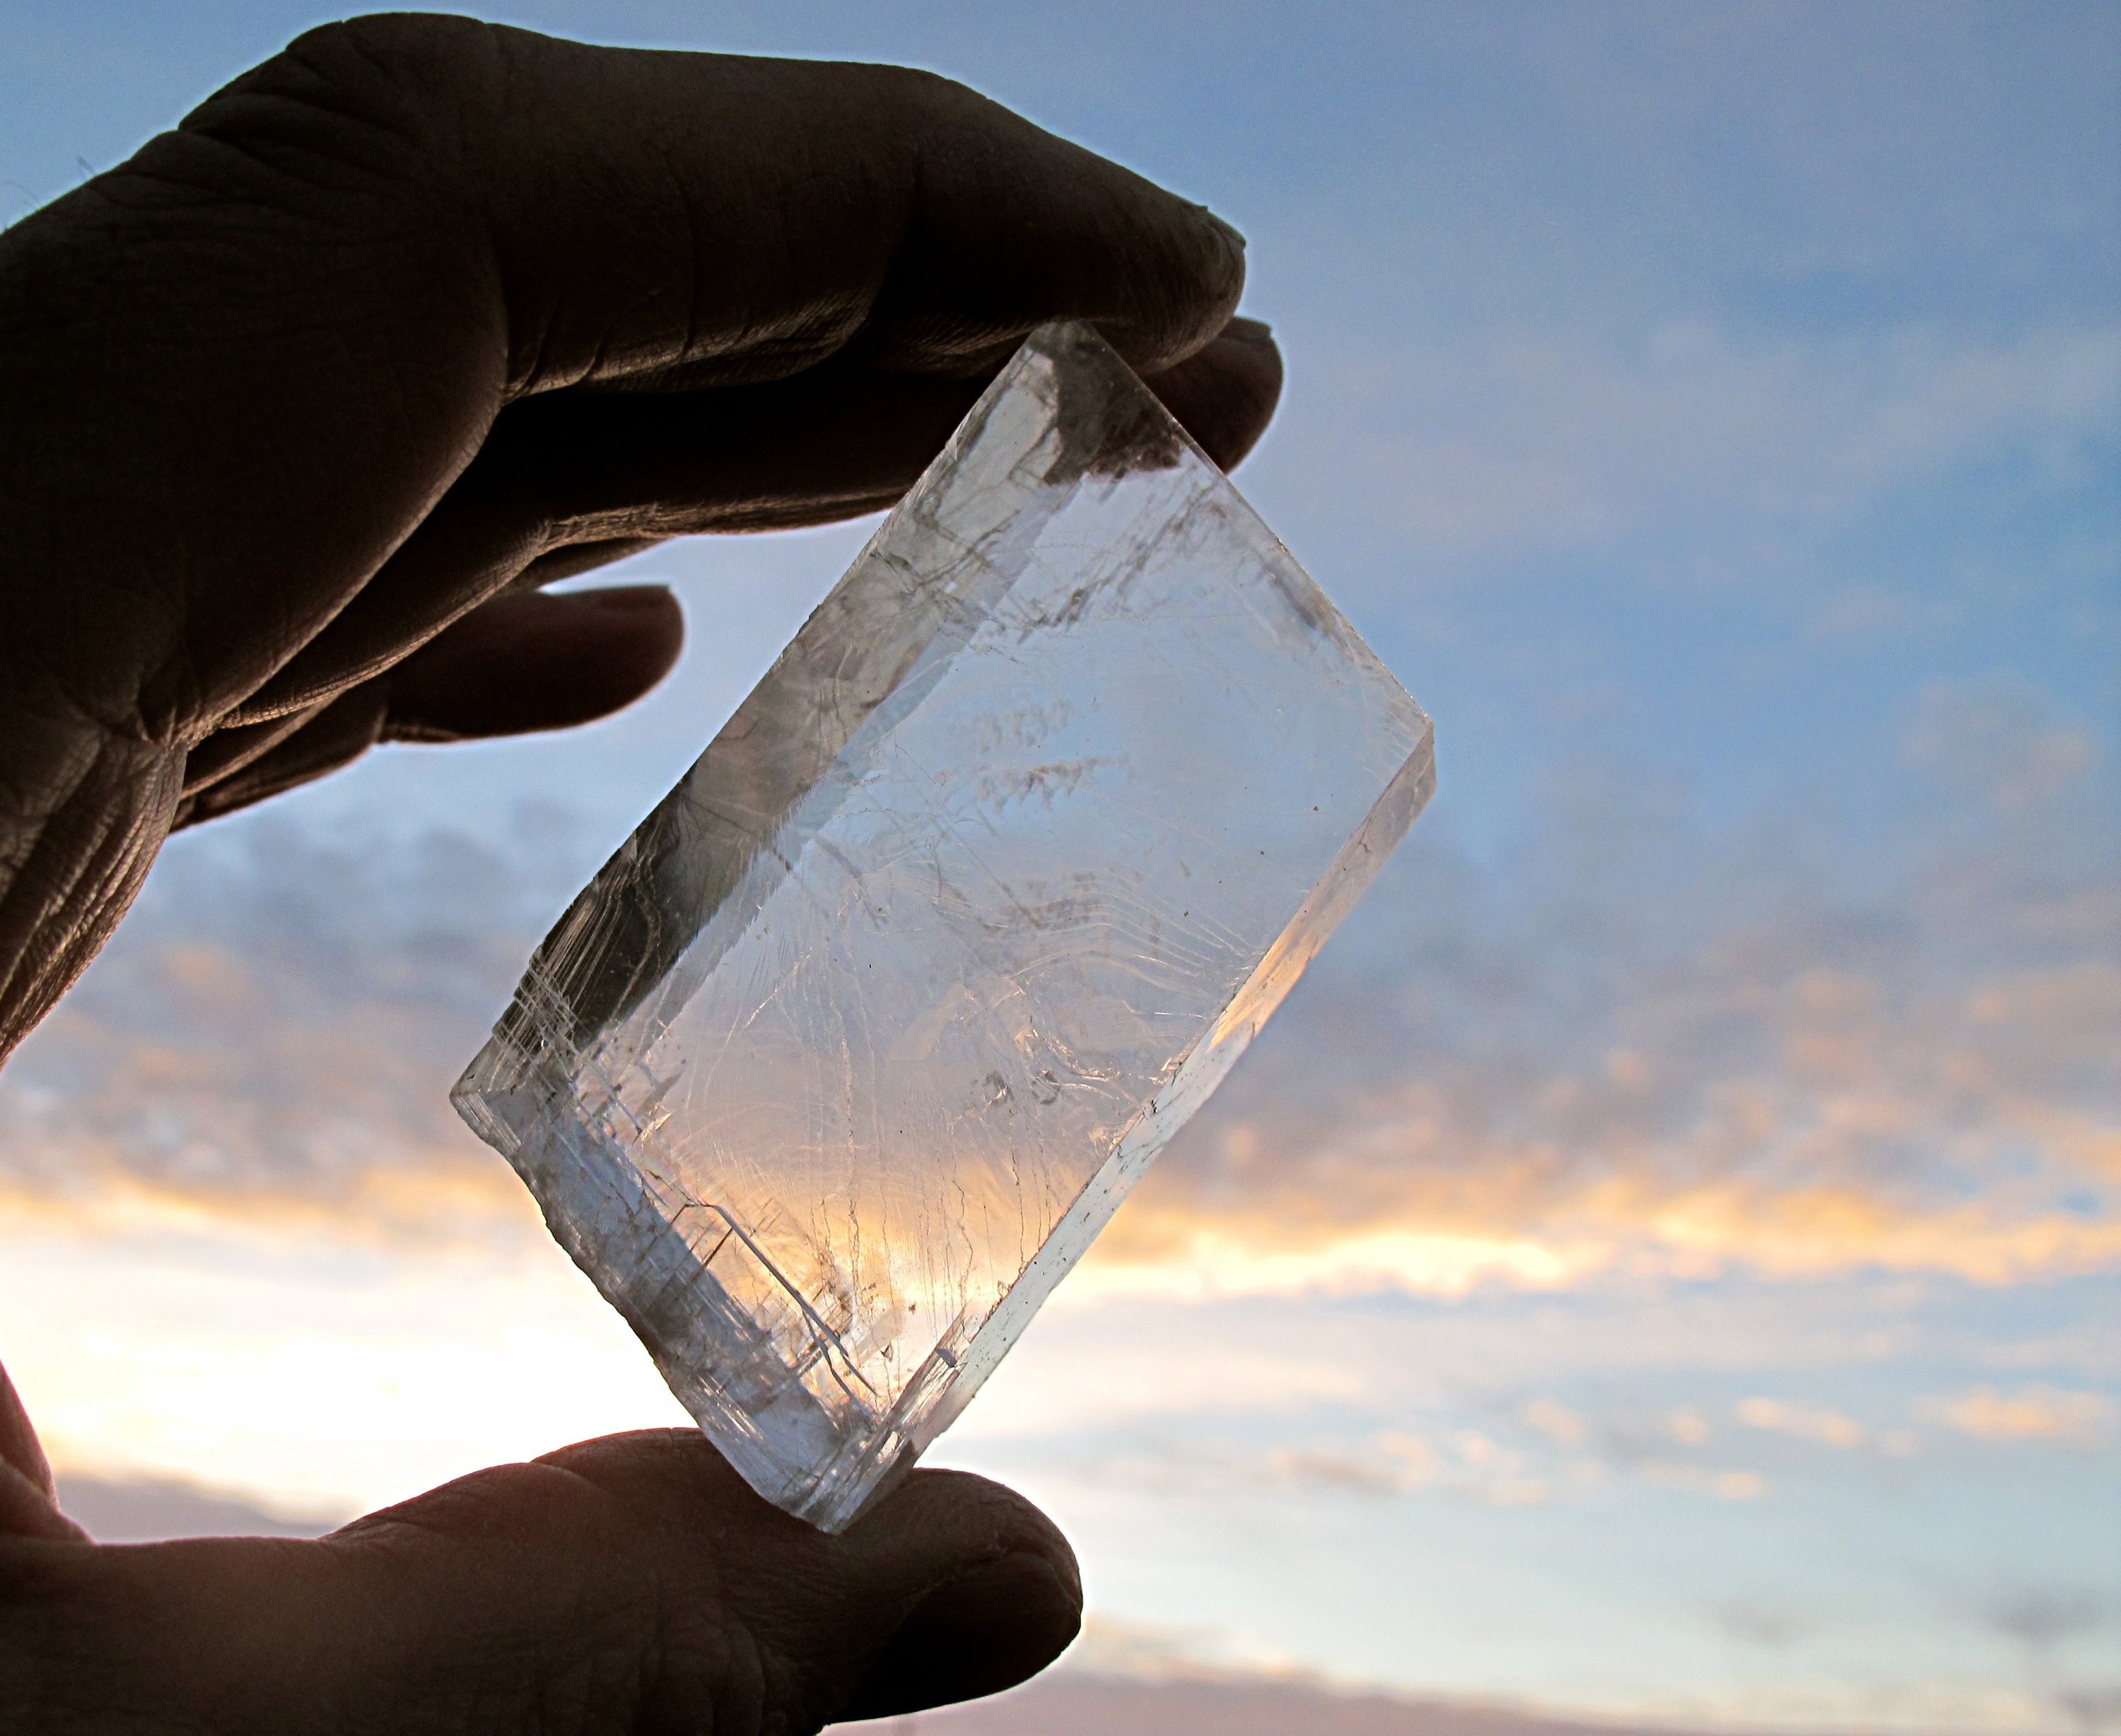
\includegraphics[width=0.5\textwidth]{espato_islandia.jpg}
%	\end{center}
%	\caption{Espato de Islandia. Variedad de piedra caliza \cite{espato}}
%	\label{fig:espato}
%\end{figure}

En la figura \ref{fig:metro} se muestra una parte del plano de la red de metro de la Comunidad de Madrid. A primera vista, uno se pierde entre tanto entresijo de líneas de colores pero si se establece una estación de origen y otra de destino, este plano facilita concretar el camino a tomar. Además, en las estaciones suele haber una gran cantidad de señalizaciones que hacen aún más fácil la localización. Entonces, si los humanos, seres inteligentes con percepción visual y capacidad de razonamiento, necesitamos localizarnos para alcanzar un objetivo, ¿porqué no lo iban a necesitar los robots? \\

\begin{figure}[h]
	\begin{center} 
	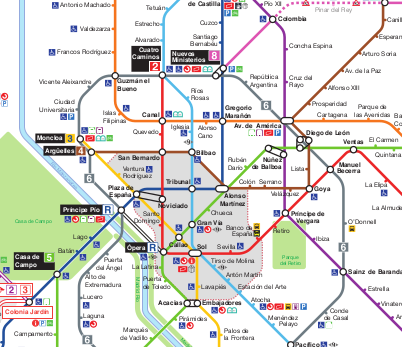
\includegraphics[width=0.4\textwidth]{plano_metro.png}
	\end{center}
	\caption{Detalle de la red de metro de la Comunidad de Madrid. \cite{metro_madrid}}
	\label{fig:metro}
\end{figure}

%\begin{figure}[H]
% \centering
%  \subfloat[Coeficiente $K=0$]{
%    \includegraphics[width=0.3\textwidth]{p6/simk0_ej1.png}}
%  \subfloat[Coeficiente $K=1$]{
%    \includegraphics[width=0.3\textwidth]{p6/simk1_ej1.png}}
% \caption{Simulación de la posición cartesiana para diferentes valores de %$K$}
% \label{fig:p6:sim_ej1}
%\end{figure}

La robótica móvil ha ido evolucionando a un ritmo vertiginoso desde que comenzó a desarrollarse. En los años sesenta se diseñó el apodado como \textit{SHAKEY} o ``el primer robot inteligente móvil del mundo'' según el IEEE (Instituto de Ingenieros Eléctricos y Electrónicos, del inglés \textit{Institute of Electrical and Electronics Engineers}). Este robot era el primero de su generación capaz de navegar en un entorno no controlado, sirviéndose de múltiples dispositivos que le proporcionaban información sobre la distribución de los elementos que le rodeaban, dándole la posibilidad al robot de evitarlos durante el trayecto \cite{shakey1}.\\

\begin{figure}[h]
	\begin{center} 
	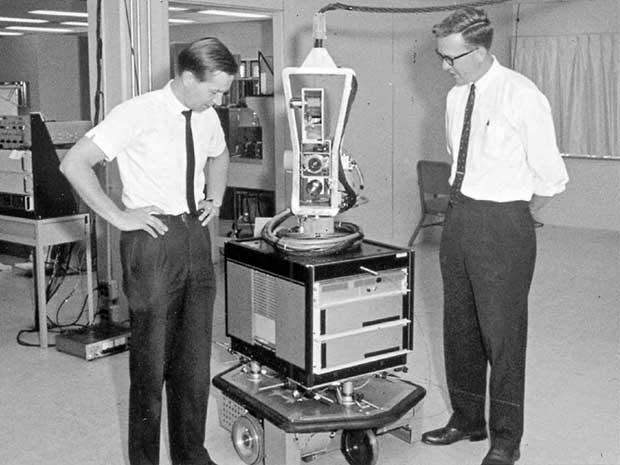
\includegraphics[width=0.8\textwidth]{shakey.jpg}
	\end{center}
	\caption{Foto tomada del robot SHAKEY en 1968. \cite{shakey2}}
	\label{fig:shakey}
\end{figure}


Un robot autónomo móvil (ARM) es un robot capaz de navegar a través de un entorno sin supervisión directa por parte de un operador humano ni la necesidad de disponer de un ruta fijada previamente. Para poder llevarlo a cabo, los robots disponen de multitud de sensores que les permiten percibir e interpretar el entorno, dotando al robot de la capacidad de navegar por el mismo evitando obstáculos, tanto fijos como móviles. Para poder realizar una navegación de alto nivel que les permita ir desde un punto origen a otro punto destino, los robots se sirven de mapas. Un mapa es una representación bidimensional del entorno. De forma general, podemos distinguir dos tipos de mapas de aplicación a la robótica: los mapas métricos y los mapas topológicos. Los mapas métricos (figura \ref{fig:mapas}, izquierda) dividen el entorno en una rejilla donde cada celda representa una probabilidad de estar ocupada o de no estarlo. Si se discretiza esa probabilidad el resultado es un mapa de ocupación, (también llamado \textit{floorplan} o ``plano de suelo'', en un ámbito menos técnico), si no, se obtiene un mapa probabilístico. El mapa métrico más simple es el formado por un conjunto de referencias visuales o \textit{landmarks} de posición conocida que ayudan al robot a estimar su posición. Los mapas topológicos (figura \ref{fig:mapas}, derecha) están basados en grafos y representan la conectividad entre cada uno de sus nodos. Existe una tercer tipo de mapa que es un híbrido entre los comentados y es el más utilizado para los robots: utilizan los grafos para la generación de trayectorias (navegación) y el mapa métrico para la localización.\\

\begin{figure}[H]
 \centering
  \subfloat[Ejemplo de mapa métrico: mapa de ocupación \cite{thrun}]{
    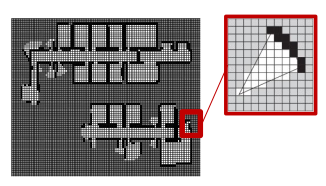
\includegraphics[width=0.35\textwidth]{mapa_ocupacion.png}}
  \hspace{2cm}
  \subfloat[Mapa topológico: líneas del metro de Málaga \cite{metro_malaga}]{
    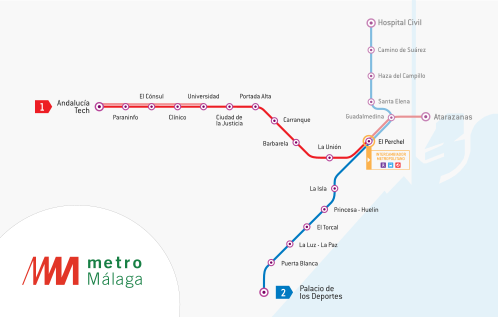
\includegraphics[width=0.3\textwidth]{metro_malaga.png}}
 \caption{Ejemplos de tipos de mapas.}
 \label{fig:mapas}
\end{figure}

Los mapas métricos más utilizados en la robótica móvil son los mapas de ocupación o \textit{floorplans}. Son generados en una primera fase de inspección del entorno, empleando los mismos sensores que luego servirán para la navegación autónoma. Tradicionalmente, estos mapas de ocupación son generados empleando un láser 2D o LIDAR (dado su gran alcance y amplio campo de visión), generando por tanto mapas bidimensionales que especifican aquellas zonas del entorno que están libres de obstáculos y por tanto susceptibles de navegación, y aquellas que no lo están. No obstante, dado que un láser 2D no puede distinguir entre los objetos detectados, los mapas de ocupación bidimensionales generados con este sensor contienen, no sólo los elementos estructurales del entorno como paredes, puertas, columnas, etc., si no que incluyen multitud de objetos como mesas y sillas, camas, cajas e incluso personas si estaban presentes en el momento de generar el mapa.\\

La inclusión de estos elementos no estructurales en el mapa de ocupación puede ocasionar problemas si se pretende utilizar ese mapa durante un largo período de tiempo. El mapa generado no estaría preparado si el entorno que representa sufre algún tipo de modificación de mobiliario, por lo que sería necesario volver a generar un nuevo mapa, con todo lo que eso conlleva. Sin ir más lejos, en la Escuela de Ingenierías Industriales hay muchos elementos que no pertenecen a la estructura del edificio que, si hoy mismo se utilizara un robot equipado con un láser 2D para generar un mapa, ocasionarían los problemas ya comentados. Estos elementos son, por ejemplo, las impresoras que hay en algunas zonas, las máquinas de refrescos y snacks, papeleras, carteles publicitarios, las nuevas mesas instaladas en la zona central, etc (figura \ref{fig:laser_vs_rgbd}). En la figura \ref{fig:laser_vs_rgbd} se muestra un ejemplo de lo que se quiere conseguir aprovechando las ventajas de los sensores RGBD frente a los láseres 2D aplicado a la Escuela de Ingenierías.\\

\begin{figure}[H]
	\begin{center} 
	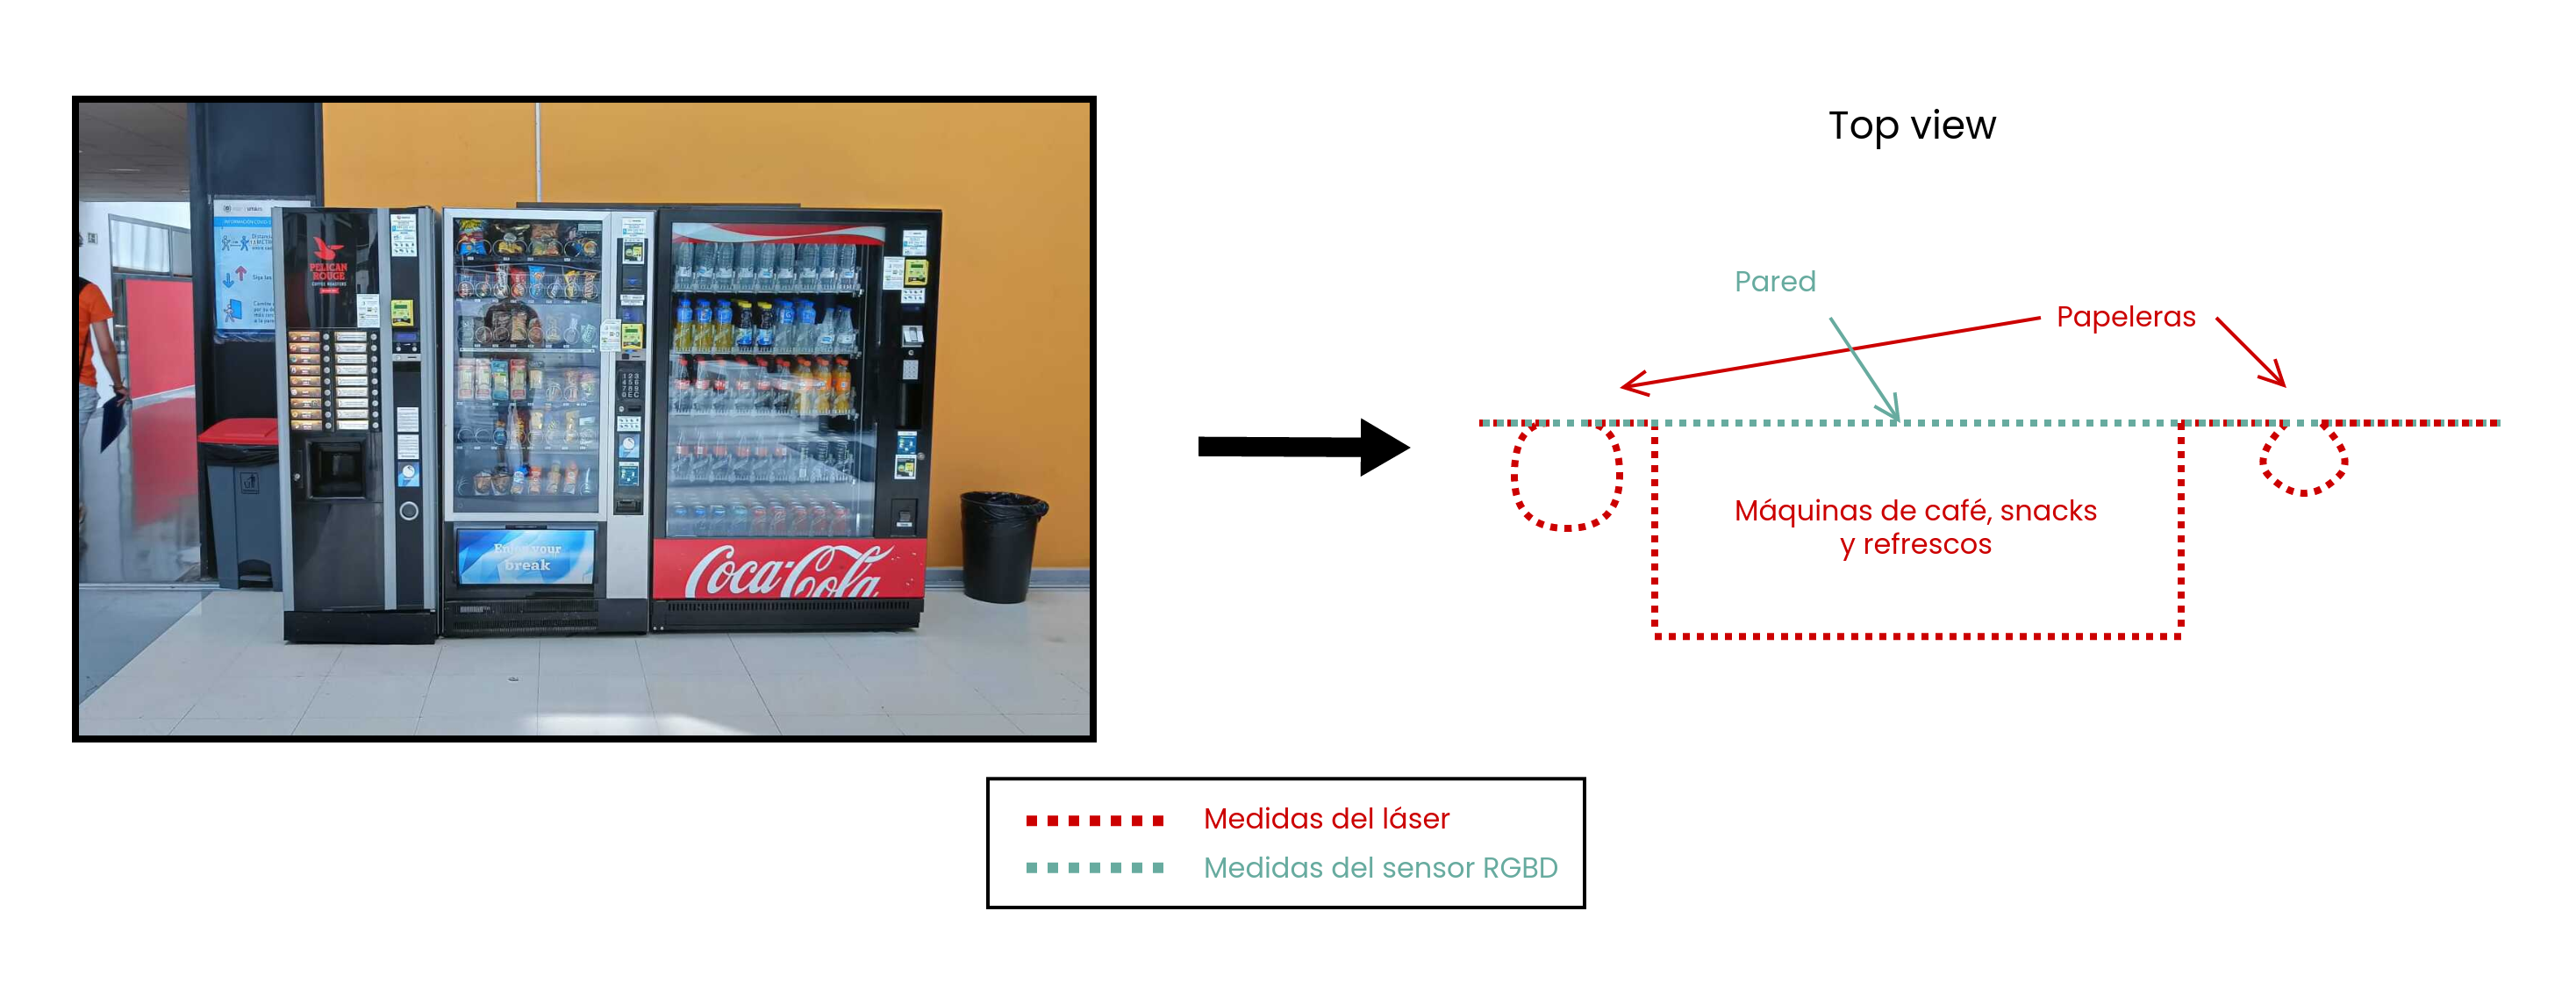
\includegraphics[width=\textwidth]{laser_vs_rgbd.png}
	\end{center}
	\caption{Comparación teórica del resultado de una medición de un láser 2D y un sensor RGBD sobre elementos presentes en la Escuela de Ingenierías Industriales.}
	\label{fig:laser_vs_rgbd}
\end{figure}

Otro ejemplo se puede ver en la figura \ref{fig:errores_laser} donde se muestra un mapa generado de un entorno virtual a través de un láser 2D de 360º. Como se puede observar hay zonas, marcadas con numeración, en las que el mapa no representa fielmente las dimensiones reales de la vivienda. De modo que, si los objetos que no forman parte de la estructura modifican su posición después de la primera fase de análisis, el mapa de ocupación generado no podría ser utilizado por el robot para la navegación. \\

\begin{figure}[h]
	\begin{center} 
	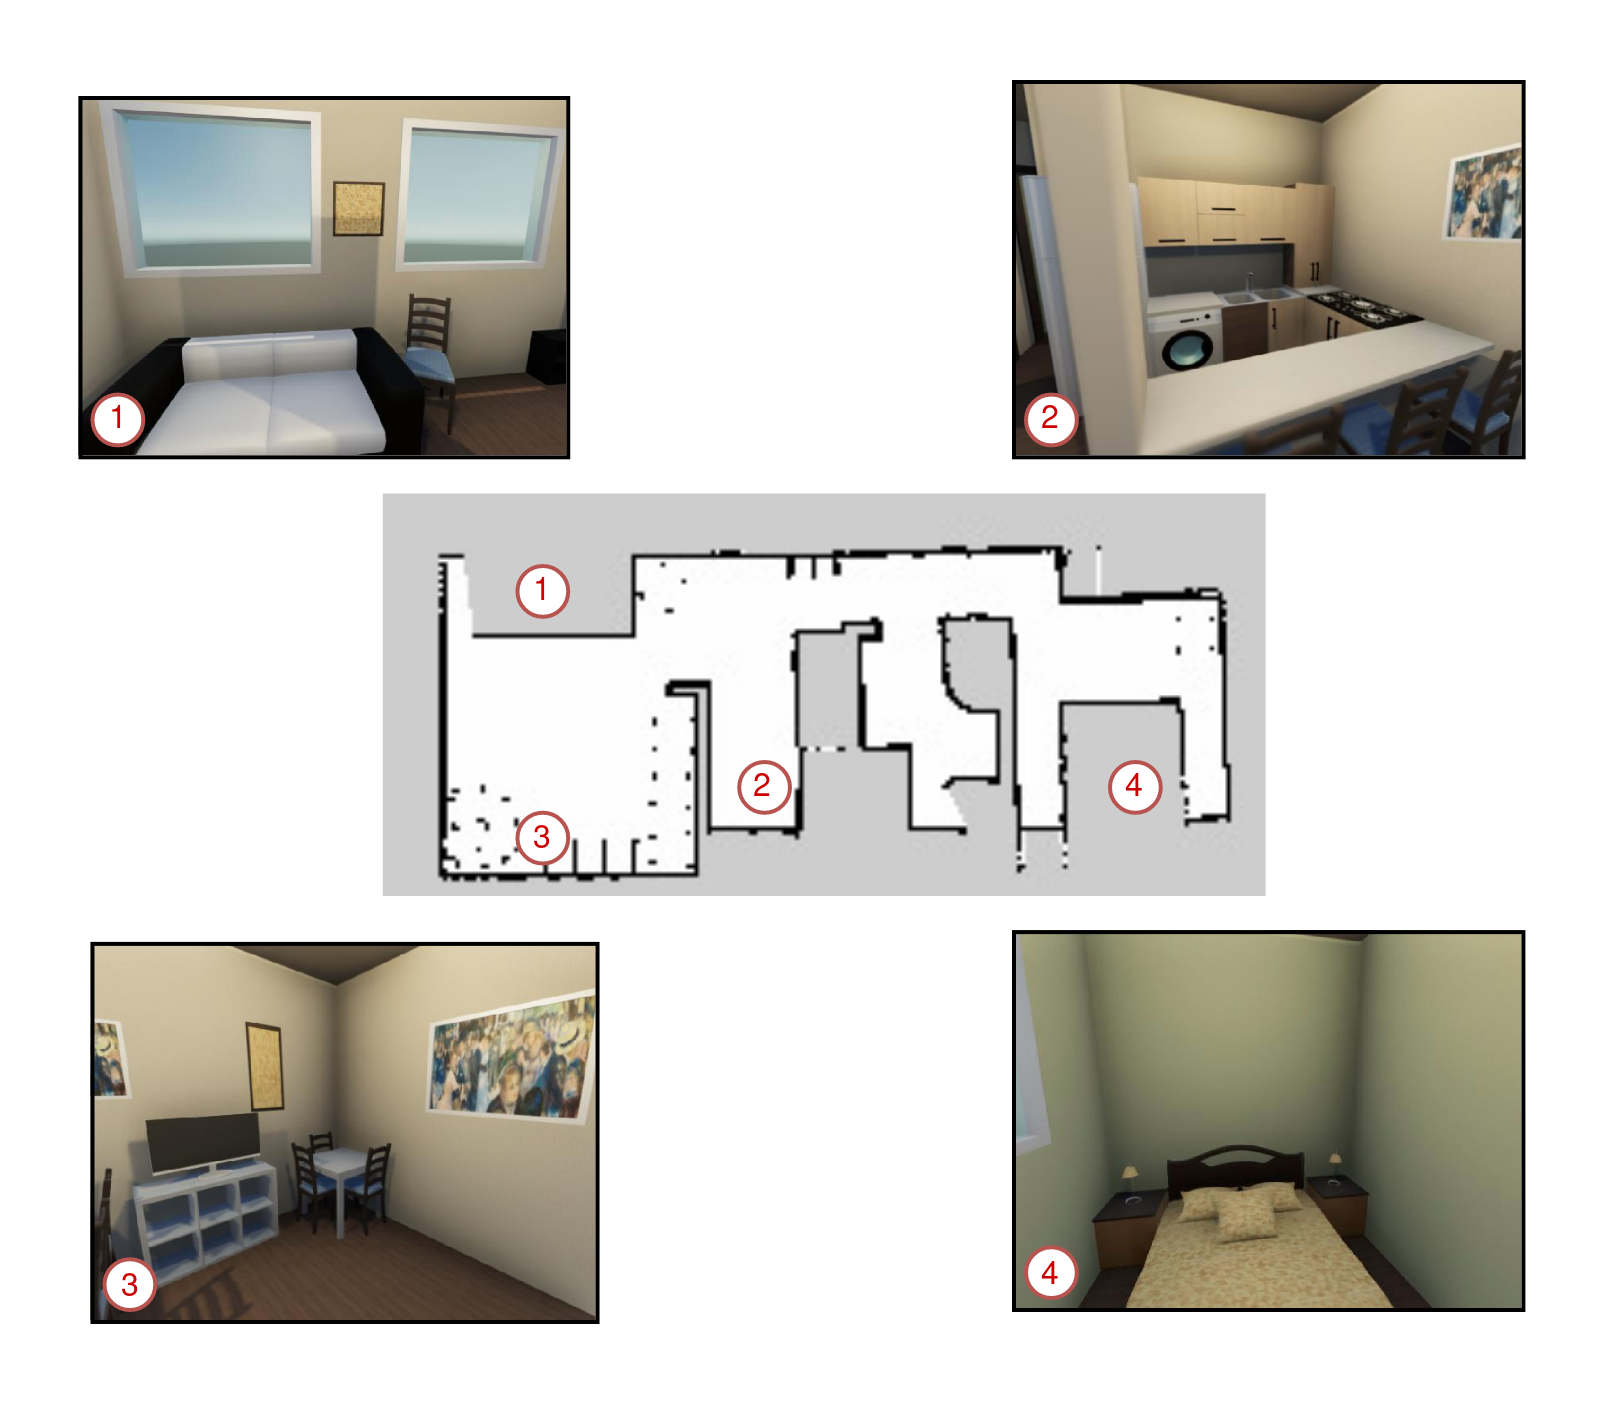
\includegraphics[width=0.6\textwidth]{IlustracionErroresMapa.png}
	\end{center}
	\caption{Mapa generado con el barrido de un láser. Las zonas enumeradas muestran que el mapa generado no representa fielmente la estructura del entorno debido a la presencia de elementos que pueden variar en su posición como un sofá, una silla, una cama, etc.}
	\label{fig:errores_laser}
\end{figure}

Dado que estos métodos de generación de mapas de ocupación mediante láser 2D sufren frente a la variabilidad en la distribución, surge la idea de utilizar otros sensores que permitan discernir entre los distintos elementos que pudieran formar parte del entorno. Los sensores RGBD son cámaras que, además de proporcionar información sobre el color, ofrecen la distancia a la que se encuentra cada píxel captado en la imagen con respecto a la cámara. Por lo tanto, ofrecen información en 3D del dominio, lo que abre más posibilidades a la hora de percibir e interpretar la información captada mediante los sensores. \\

En este proyecto se pretende analizar una posible solución al problema de fiabilidad en la representación de los mapas de ocupación realizados con sensores LIDAR mediante el uso de sensores RGBD para generar \textit{floorplans} fieles a la estructura invariable del entorno. Entre las utilidades de conseguir un mapa sin los objetos móviles, las más destacadas son:

\begin{itemize}

	\item La más importante es la posibilidad de tener un mapa que permita al robot localizarse aún con los cambios que puedan surgir a lo largo del tiempo en los elementos que conforman el entorno. Así se evita tener que generar un nuevo mapa cada vez que surja algún cambio significativo.
	\item En aplicaciones de realidad aumentada para el diseño de interiores, este sistema permitiría obtener las dimensiones reales de la vivienda y así tener una idea en primera persona del cambio de mobiliario o de una nueva organización del mismo.
	\item Normalmente existe una clara disparidad entre el plano de una vivienda o de un edificio diseñado por el arquitecto y el producto final. Con este mapa generado sería posible comparar y obtener un plano fiel a la realidad y así validar las dimensiones reales de la infraestructura.

\end{itemize}



\section{Objetivo}

Dado que los robots utilizan los mapas de ocupación o \textit{floorplans} para localizarse y navegar en un entorno, es necesario que éstos sean lo más fiel posible a la estructura real del edificio o de la vivienda. Esto resulta imposible si durante la fase de obtención del mapa existen elementos que no pertenecen a la infraestructura, ya que provocan que el mapa resultante no sea fiel a las dimensiones reales del entorno.\\

Debido a la necesidad y utilidad de obtener mapas de ocupación sin elementos cambiantes, el objetivo de este trabajo es utilizar la información proporcionada por sensores RGBD para la generación de \textit{floorplans}, solucionando problemas de variabilidad en el entorno que perjudican seriamente la fiabilidad del mapeado mediante sensores láser.\\

Se obtendrá información acerca de la profundidad de los píxeles captados y se escogerán aquellos puntos menos restrictivos (más alejados) para generar un láser artificial que permita la creación del mapa de ocupación mediante algoritmos de mapeado.\\

Paralelamente, se utilizará un modelo entrenado de inteligencia artifical, YOLO, para detectar los elementos de la imagen de color y así llevar un registro de los objetos que se ha encontrado el robot en su trayectoria.\\

Finalmente, se hará una comparativa de los resultados obtenidos únicamente con el LIDAR con los obtenidos mediante el procesamiento de la información de la cámara. Además se hará un estudio de los objetos detectados durante el mapeado y de la fiabilidad del modelo de detección. \\

\section{Estructura del documento}

Este documento está dividido en cuatro partes. En la primera parte se hará una introducción al contexto del proyecto y se explicará por qué se ha desarrollado.\\

La segunda parte consta de tres capítulos. En el primero de ellos se expondrán las herramientas utilizadas y se explicarán brevemente cómo se utilizan y porqué se han escogido. En un segundo capítulo, el más importante, se desarrollará el trabajo y se explicará cómo se ha llevado a cabo. En el tercer y último capítulo se expondrán los resultados y se compararán con los ideales, comentando sus diferencias y problemas encontrados.\\

En la tercera parte se mostrarán las conclusiones obtenidas tras la consecución del proyecto y se comentarán algunas posibles líneas de trabajo abiertas de cara al futuro, así como posibles mejorías que se pudieran implementar. \\

En una cuarta y última parte se sitúan los apéndices del proyecto. En el primero se explica el software que se ha utilizado de apoyo pero que no se ha mencionado en los capítulos anteriores. En el segundo apéndice se expone el código de los nodos que han sido diseñados expresamente para este trabajo.\\





























\part{Desarrollo}

\chapter{Herramientas utilizadas}

\section{Robotic Operating System}

Robot Operating System (ROS) es un framework para el desarrollo de software de robots. Se desarrolló originariamente en 2007 por el Laboratorio de Inteligencia Artificial de Stanford para dar soporte a su proyecto STAIR2\footnote{STAIR (Stanford Artificial Intelligence Robot) es un proyecto llevado a cabo por la Universidad de Stanford para desarrollar robots capaces de navegar en entornos indoor e interactuar con objetos y personas mediante inteligencia artificial. Para su versión 2.0 desarrollaron el framework de ROS. \cite{stair}} \cite{stair_paper}. Es software libre bajo términos de licencia BSD\footnote{La licencia BSD es la licencia de software libre otorgada principalmente para los sistemas BSD (Berkeley Software Distribution). Es una licencia permisiva que permite la redistribución libre. \cite{licencia}} que, pese a no ser un sistema operativo, provee los servicios estándar de éstos entre los que se incluyen la abstracción del hardware, el control de dispositivos de bajo nivel, la implementación de funcionalidad de uso común, el paso de mensajes entre procesos y el mantenimiento de paquetes. Está basado en una arquitectura de grafos donde el procesamiento toma lugar en los nodos que pueden recibir, mandar y multiplexar mensajes de sensores, control, estados, planificaciones y actuadores, entre otros.\\


\subsection{Arquitectura de la comunicación mediante ROS}

La unidad básica de una comunicación en ROS es el \textit{nodo}. Un nodo es un programa diseñado en Python o C++ que se comunica con otros nodos principalmente mediante \textit{topics}. Cuando varios nodos se complementan para cumplir una determinada función, se suelen agrupar en paquetes. Un paquete contiene, entre otras cosas, el nodo o los nodos que lo conforman, las dependencias necesarias para la ejecución de alguno de sus nodos, información acerca del propio paquete, etc. ROS tiene sus propios paquetes incluidos de forma estándar con la instalación pero además se pueden instalar paquetes de terceros, desarrollados por otros usuarios.\\

Existe un nodo especial, llamado nodo \textit{master}, que se encarga de registrar las direcciones de cada nodo y qué y dónde publica o se suscribe. Además, se encarga de alojar el servidor de parámetros, accesibles y modificables en cualquier momento. Es necesario lanzar este nodo previamente al lanzamiento de cualquier otro. \\

Los topics son el método más común de comunicación entre nodos. Está basado en el modelo de publicador/suscriptor. Los nodos pueden publicar (Publisher) o recibir (Subscriber) mensajes de un único tipo, establecidos por el nodo publicador. En un mismo topic pueden publicar y suscribirse tantos nodos se necesiten\footnote{Realmente, ROS especifica que no existe límite de nodos suscritos a un mismo topic. Sin embargo, se ha demostrado que a partir de 10 nodos, la fiabilidad se ve reducida y la latencia aumentada de forma significativa, pudiendo incluso ocasionar que algunos mensajes no sean recibidos por algunos suscriptores. \cite{issue}}. \\

Otro método de comunicación son los servicios o \textit{services}. Están basados en un modelo de llamada/respuesta. Mientras que los topics permiten a los nodos obtener continuas actualizaciones de datos, los servicios solo ofrecen respuesta tras ser llamados. Permiten la inclusión de parámetros tanto en la solicitud como en la respuesta al servicio. Este método es bloqueante, es decir, el nodo solicitante queda bloqueado al momento de enviar la solicitud hasta que reciba una respuesta, por lo que están pensados para ser utilizados en tareas que no ocupen mucho tiempo.\\

El otro método de comunicación que existe en ROS son las acciones o actions, pensadas para tareas que necesiten una gran cantidad de tiempo para poder ser realizadas. Las acciones funcionan con un modelo cliente/servidor. A diferencia que los servicios, las acciones no son bloqueantes y permiten ser canceladas mientras se están ejecutando.\\

Como se ha comentado, el método más usual de comunicación es a través de topics, donde los nodos envían y reciben información continuamente, sin peticiones ni esperas. Los servicios y acciones se utilizan en función de los requerimientos del software a desarrollar.\\

\begin{figure}[H]
 \centering
  \subfloat[Topics]{
    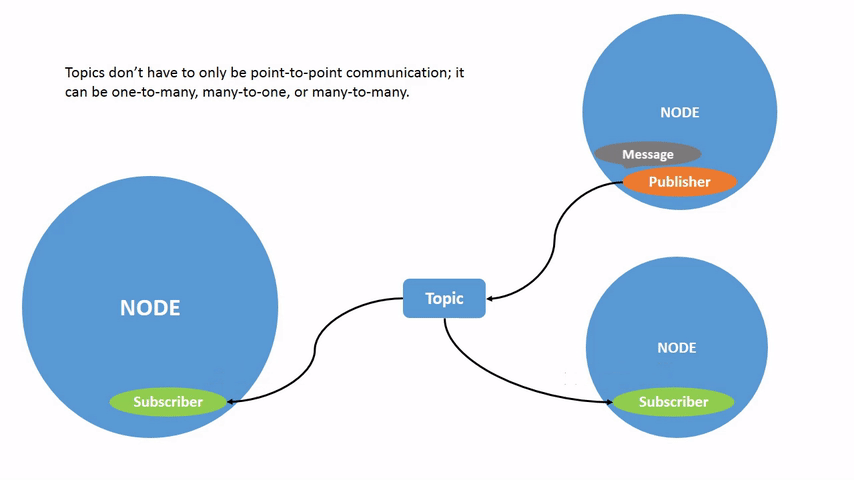
\includegraphics[width=0.5\textwidth]{exp_topics.png}}
  \hspace{0.5cm}
  \subfloat[Services]{
    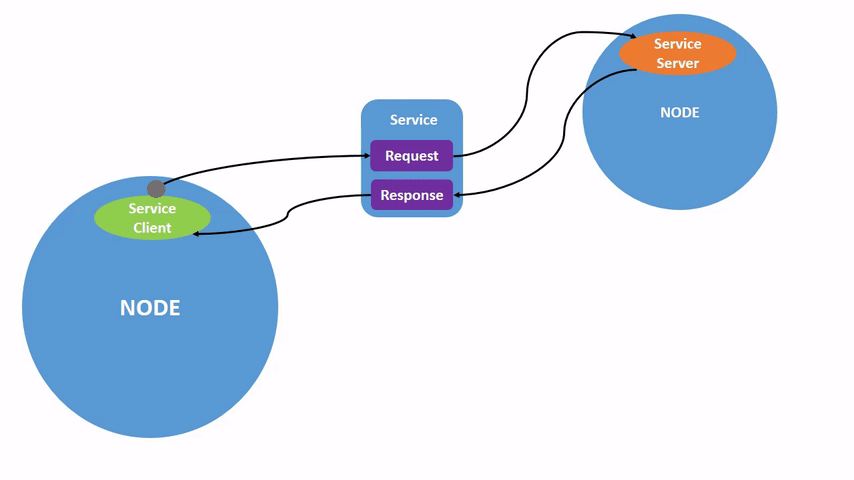
\includegraphics[width=0.5\textwidth]{exp_services.png}}
  \subfloat[Actions]{
    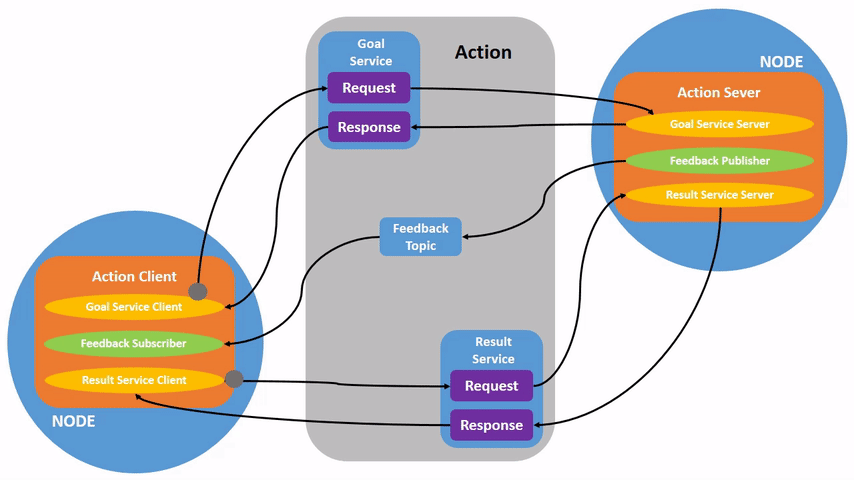
\includegraphics[width=0.5\textwidth]{exp_actions.png}}
 \caption{Mecanismos de comunicación en ROS. (a) Topics, (b) Servicios y (c) Acciones}
 \label{fig:comm}
\end{figure}

ROS también implementa una herramienta muy útil a la hora de probar los programas que se desarrollan. Un \textit{rosbag} de ROS es una herramienta que permite capturar todos los mensajes que se publican por determinados topics para luego reproducirlos. Esto permite ejecutar el robot una única vez capturando todos los topics y luego reproducir los mensajes de estos topics cuantas veces queramos, permitiendo probar los nodos que se estén desarrollando sin tener que hacerlo directamente sobre el robot. Toda esta información se guarda en un archivo .bag. \cite{roswiki}\\

\subsection{¿Por qué ROS?}

La comunidad robótica ha evolucionado considerablemente a lo largo de los años. Pese a  este rápido progreso, los robots aún presentan auténticos desafíos para los desarrolladores de software. ROS nace precisamente para facilitar muchas de las dificultades que surgen en la comunicación entre los distintos elementos que conforman un robot.\\

Muchos de los sistemas robóticos modernos necesitan de un sistema de comunicaciones que sirva de enlace entre los diferentes procesos. Estos procesos suelen dividirse en varias computadoras, lo que complica aún más la comunicación. Las diferentes vías de comunicación que ROS pone a disposición brindan a los desarrolladores infinidad de posibilidades.\\

Pero la que es quizá la mayor ventaja de ROS frente a otros frameworks y software especializado en robótica es la gran comunidad que tiene detrás. Existen miles de usuarios que contribuyen continuamente con nuevos paquetes que implementan funcionalidades de todas las ramas de la robótica, lo que abre un abanico de opciones para el desarrollador, reduciendo en gran medida la curva de aprendizaje.\\

\section{Mapas de ocupación}

Un mapa o rejilla de ocupación es una representación bidimensional del entorno que se almacena en el robot para realizar tareas de navegación. Está formado por celdas que discretizan el entorno y determinan si una porción del espacio está ocupado o no. Generalmente, las celdas ocupadas se representan con el color negro, y las celdas libres con el blanco.\\

Para generar estos mapas, se utiliza la información obtenida de los diferentes sensores que conforman el robot, como pueden ser infrarrojos, cámaras RGBD, sónares o, los más utilizados, láseres 2D. Independientemente de la fiabilidad del sensor, no es posible establecer con certeza si una celda está ocupada o no. En la generación de estos mapas, típicamente se establecen tres suposiciones: una celda puede estar libre u ocupada, cada celda es independiente a las demás y el entorno es estático. Para estimar las distribuciones de probabilidad de cada celda se utiliza generalmente un Filtro de Ocupación Bayesiano (BOF) \cite{occupancy_grid}.\\

\begin{figure}[h]
\begin{center} \label{fig:occ_map}
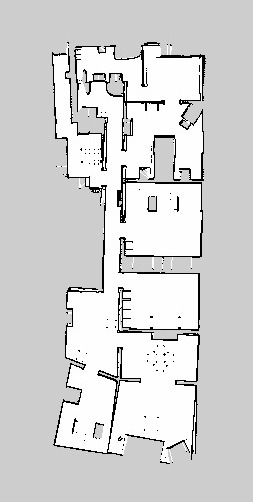
\includegraphics[width=0.4\textwidth, angle=90]{occ_map_img.jpg}
\end{center}
\caption{Ejemplo de mapa de ocupación en formato \texttt{.pgm}}
\end{figure}

\section{Sensores RGBD}

Las cámaras RGBD son sensores visuales que, además de ofrecer información de color del entorno, proporcionan la distancia a la que se encuentra cada píxel de la imagen. Son cámaras a color comunes a las que se le añade un sensor de profundidad (normalmente, sensores infrarrojos) junto con un procesamiento que les permite percibir e interpretar la distancia a la que se sitúan los diferentes elementos del entorno que estén dentro de su campo de visión.\\

\begin{figure}[h]
	\begin{center} 
		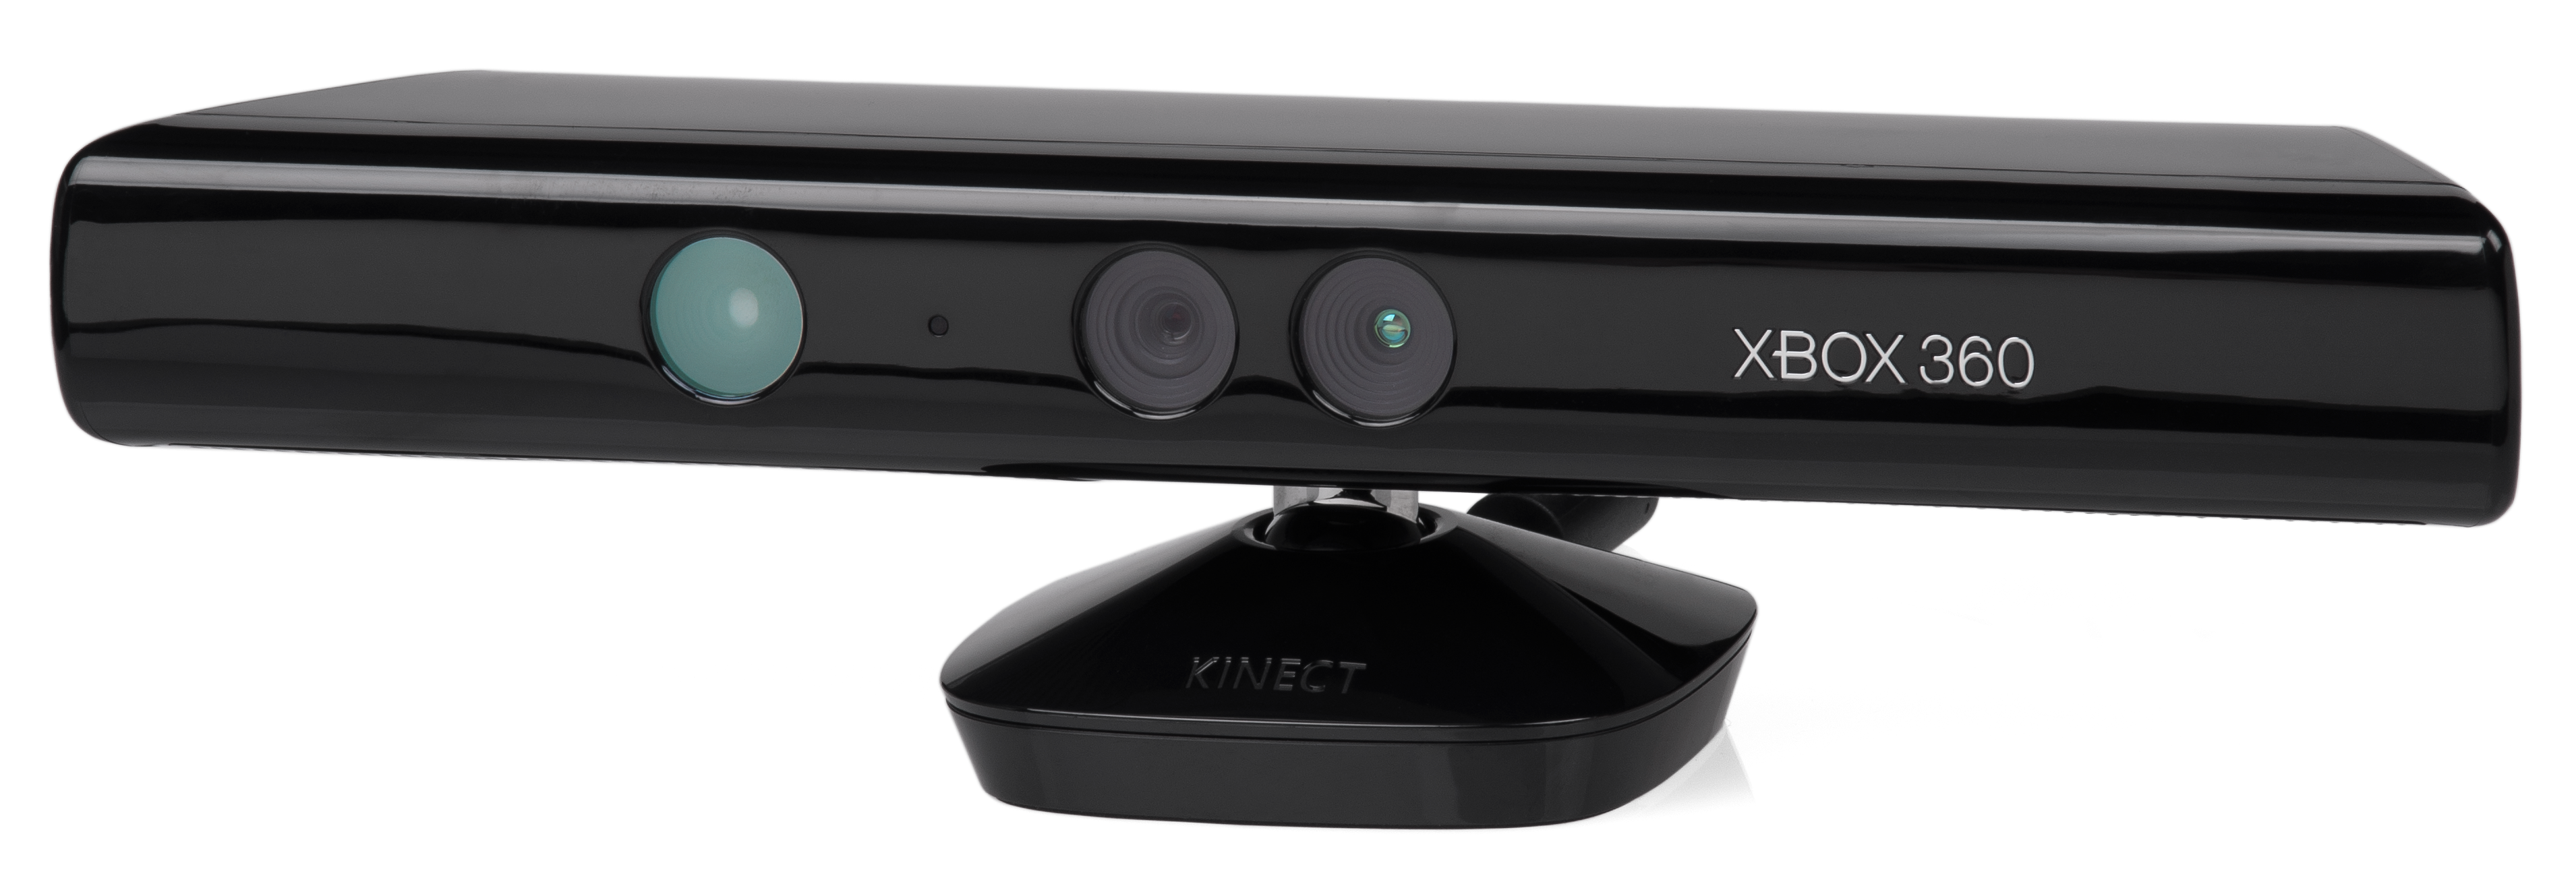
\includegraphics[width=0.5\textwidth]{kinect_img.png}
	\end{center}
	\caption{Fotografía del sensor Microsoft Kinect V1, lanzado como complemento de la videoconsola Xbox360 en 2010 \cite{kinectv1}}
	\label{fig:kinect}
\end{figure}

Algunos de los fabricantes más importantes de este tipo de sensores son Microsoft, con la conocida Kinect; ASUS, IFM, StereoLabs, Intel, Orbbec, etc.\\

\subsection{Imagen de profundidad}

La imagen de profundidad, al igual que cada uno de los canales de color RGB, es una matriz donde cada valor representa un nivel de gris asociado a una distancia y está referido a cada uno de los píxeles que componen la imagen. Las dimensiones de esta imagen vendrán determinadas por la resolución de la cámara, es decir, si por ejemplo la resolución de la cámara es de 640x480 píxeles, la matriz tendrá 480 filas y 640 columnas. \\

\begin{figure}[H]
	\begin{center} 
		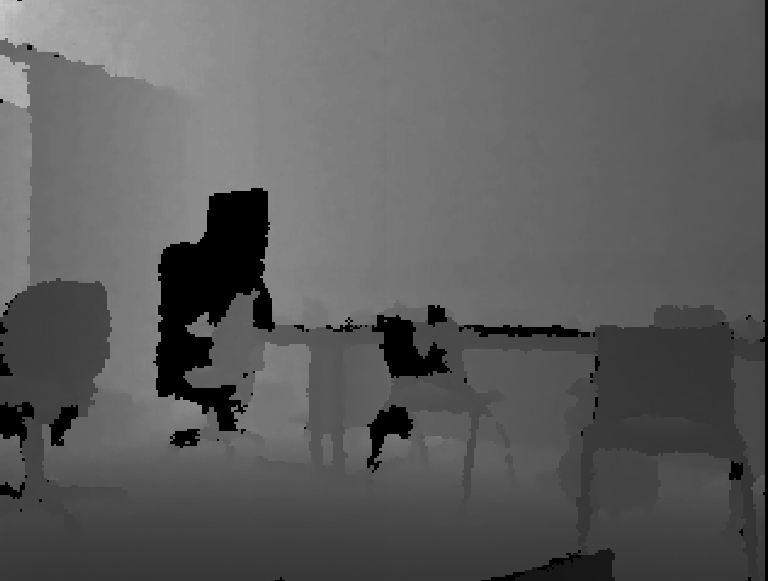
\includegraphics[width=0.7\textwidth]{depth_img.png}
	\end{center}
	\caption{Ejemplo de imagen de profundidad \cite{depthimage}. Generalmente, los objetos más alejados se representan en tonos más claros, mientras que los tonos más oscuros representan las zonas más cercanas. Las zonas donde es un color negro puro son zonas de ``no información'' de las que el sensor no puede concretar ninguna distancia}
	\label{fig:depth}
\end{figure}


El valor de distancia para cada píxel establece un nivel de gris. Generalmente, los objetos situados más alejados del sensor tendrán valores más claros, mientras que a los más cercanos se le asignan valores más oscuros. Esta información se decodifica para obtener así la información absoluta en distancia, típicamente en metros o milímetros, dependerá de la codificación con la que la cámara envía la información.\\

\section{Nubes de puntos}

Una nube de puntos o pointcloud es un conjunto de vértices en un sistema de coordenadas tridimensional. Estos vértices se identifican habitualmente como coordenadas X, Y y Z y son representaciones de la superficie externa de un objeto. Se crean a partir de escáneres láser tridimensionales o imágenes de profundidad.\\

Las nubes de puntos tienen infinidad de aplicaciones como la elaboración de modelos 3D en CAD de piezas fabricadas, la inspección de calidad en metrología y muchas otras en el ámbito de la visualización, animación, texturización y aplicaciones de personalización masiva.\\

\begin{figure}[h]
	\begin{center} 
		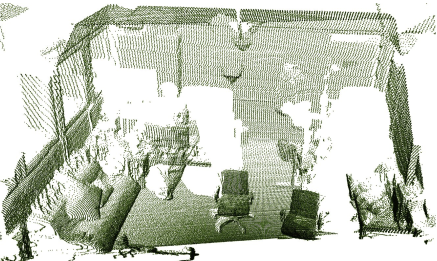
\includegraphics[width=0.7\textwidth]{pointcloud-img.png}
	\end{center}
	\caption{Ejemplo de una nube de puntos coloreada representando a una estructura}
	\label{fig:pc}
\end{figure}

\section{YOLO: You only look once}

You only look once (YOLO) es un sistema en tiempo real de detección de objetos basado en rede neuronales convolucionales y deep learning. Su principal característica y la que le distingue de otros modelos para la detección de objetos es que solo requiere visualizar una única vez la imagen (haciendo honores a su acrónimo). Esta propiedad le permite ser más rápido que los modelos competidores permitiendo la detección en tiempo real en vídeos de hasta 30 FPS. Según comentan sus creadores, es 1000 veces más rápido que R-CNN y 100 veces más rápido que Fast R-CNN.  \cite{yolo} \\

\begin{figure}[H]
	\begin{center} 
		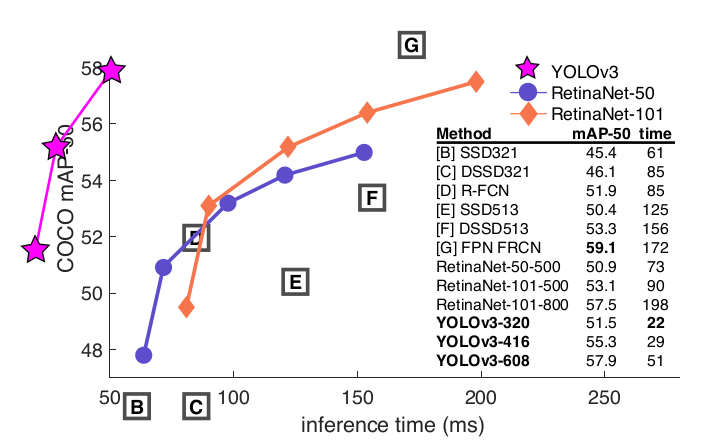
\includegraphics[width=0.8\textwidth]{grafica_rendimiento_yolov3.png}
	\end{center}
	\caption{Comparación de YOLO con otros modelos mostrando el tiempo de inferencia (eje X) y la métrica COCO mAP-50 (eje Y). Se puede ver como YOLO tiene unos tiempos de inferencia muchos menores que la mayoria de algoritmos, mantieniendo una buena puntuación en la métrica}
	\label{fig:rend}
\end{figure}

El procedimiento llevado a cabo por YOLO es sencillo. Primero divide la imagen en una cuadrícula de $S \times S$ y en cada una de estas celdas precide N posibles bounding boxes y calcula su probabilidad. Tras el cálculo, se eliminan aquellas que no superen un umbral de probabilidad. A las bounding boxes restantes, se les somete a un proceso de supresión de no máximos con el objetivo de eliminar los objetos que fueron detectados por duplicado, obteniéndose el resultado de la figura \ref{fig:proced}.\\

\begin{figure}[h]
	\begin{center} 
		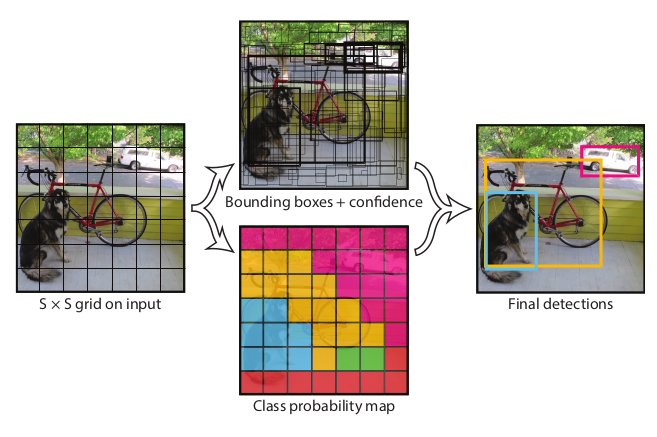
\includegraphics[width=0.8\textwidth]{yolo_proced.png}
	\end{center}
	\caption{Procedimiento llevado a cabo por YOLO. Divide la imaegn en una rejilla de $S \times S$ y predice las bounding boxes junto con sus probabilidades. Las bajas probabilidades se eliminan y, posteriormente las cajas duplicadas, obteniendo así la detección final}
	\label{fig:proced}
\end{figure}

YOLO es fácilmente implementable en ROS gracias al paquete darknet\_ros, que permite utilizarlo tanto en GPU como en CPU. La ventaja de usar la GPU para lanzar el modelo es que es 500 veces más rápido que utilizando la CPU. Para utilizar la GPU es necesario instalar el software CUDA de Nvidia. Más información sobre este software en el apéndice \ref{apendA.cuda}.\\

\subsection{Redes neuronales convolucionales}

Una red neuronal o NN (del inglés, \textit{Neural Network}) es un modelo simplificado que emula el modo en que el cerebro humano procesa la información, simultaneando multitud de unidades de procesamiento interconectads, emulando una versión artificial de las neuronas. Las neuronas se organizan en capas. En una red neuronal hay tres tipos de capas: la capa de entrada, unas o varias capas ocultas y la capa de salida. Las neuronas se conectan con las neuronas de la siguiente capa mediante ponderaciones, propagando los datos de entrada a la salida. La red aprende examinando los registros individuales, generando una predicción para cada registro y, en caso de realizad una predicción incorrecta, corriegiendo las ponderaciones. Este procedimiento, conocido como entrenamiento, se repite hasta alcanzar criterios de finalización.  Una vez la red es entrenada, puede aplicarse en casos en los que no conoce el resultado para obtener, en función del tipo y de la cantidad de entrenamiento, unos resultados satisfactorios o erróneos. \cite{nn}\\

\begin{figure}[h]
	\begin{center} 
		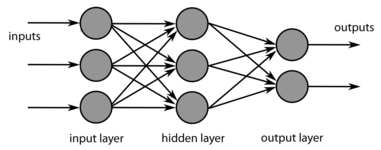
\includegraphics[width=0.6\textwidth]{nn.png}
	\end{center}
	\caption{Capas de una red neuronal artifical. Capa de entrada (izquierda), capas ocultas (centro) y capa de salida (derecha) \cite{foto_nn}}
	\label{fig:nn}
\end{figure}

Una red neuronal convolucional o CNN (del inglés, \textit{Convolutional Neural Network}) son un tipo de NN donde las neuronas corresponden a campos receptivos de una manera muy similar a las neuronas de la corteza visual primaria de un cerebro humano. Es una variación del perceptrón multicapa\footnote{El perceptrón multicapa es una red neuronal artificial formada por múltiples capas, de tal forma que tienen capacidad para resolver problemas que nos son linealmente separables. \cite{perceptron}}, muy efectiva para tareas de visión artificial. Las capas ocultas de una CNN está nespecializadas en determinadas funciones de forma que las primeras capas pueden detectar líneas o curvas y se van especializando hasta llegar a capas más profundas que reconocen formas complejas como rostros o siluetas. \cite{cnn} \\

\section{Pandas y Matplotlib}

\textit{Pandas} es una librería de código abierto de Python utilizada en el ámbito del \textit{Data Science} y \textit{Machine Learning}. Ofrece estructuras muy poderosas y flexibles que facilitan la manipulación y el tratamiento de los datos. \cite{pandas}\\

\textit{Matplotlib} es una librería de Python diseñada para la creación de visualizaciones estáticas, animadas e interactivas. Permite la creación y personalización de todo tipo de representaciones gráficas de datos, como gráficos de barras, sectores circulares, puntos, etc.\cite{matplotlib}\\

Estas herramientas, en combinación con la librería \textit{Numpy} (diseñada para el manejo de arreglos con maytor rendimiento), son las herramientas más utilizadas en el ámbito de la ciencia de datos, ofreciendo multitud de herramientas y funcionalidades que simplifican el manejo de datos.\\



\chapter{Diseño e implementación}

Para implementar el sistema que nos permita obtener estos mapas de ocupación a partir de la imagen de profundidad generada por una cámara RGBD, se utilizarán una serie de nodos de ROS. Algunos de estos paquetes y nodos son proporcionados por la comunidad de usuarios de ROS. Otros son diseñados expresamente para este proyecto.\\

Primeramente se realizará una visión general de todo el conjunto de nodos y paquetes. Se explicará el camino que llevará la información y las formas que tienen los nodos de comunicarse.\\

Sobre los paquetes de terceros, se hará una breve explicación sobre la función que tienen de fábrica y la funcionalidad que se le han dado en este trabajo, así como el modo de comunicación con todo el árbol de nodos.\\

\section{Vista general del sistema}

Como se ha comentado, el objetivo es transformar la imagen de profundidad que se obtiene de un sensor RGBD en un láser artificial para generar un mapa de ocupación. En otro proceso, simultáneamente o de forma asíncrona, se generará un archivo de texto o CVS con los elementos detectado por YOLO de la imagen de color para tener un registro y poder analizarlo. En la figura \ref{fig:esq_general} se muestra el árbol de nodos y topics de todo el sistema. Los nodos que han sido diseñados para este proyecto se muestran en color azul. Los nodos que han sido obtenidos de otras fuentes pero han necesitado de alguna modificación en su código se muestran en color naranja. Los nodos que no se han modificado se muestran en blanco. Los topics se representan con una caja de color blanco.\\

\begin{figure}[h]
	\begin{center} 
		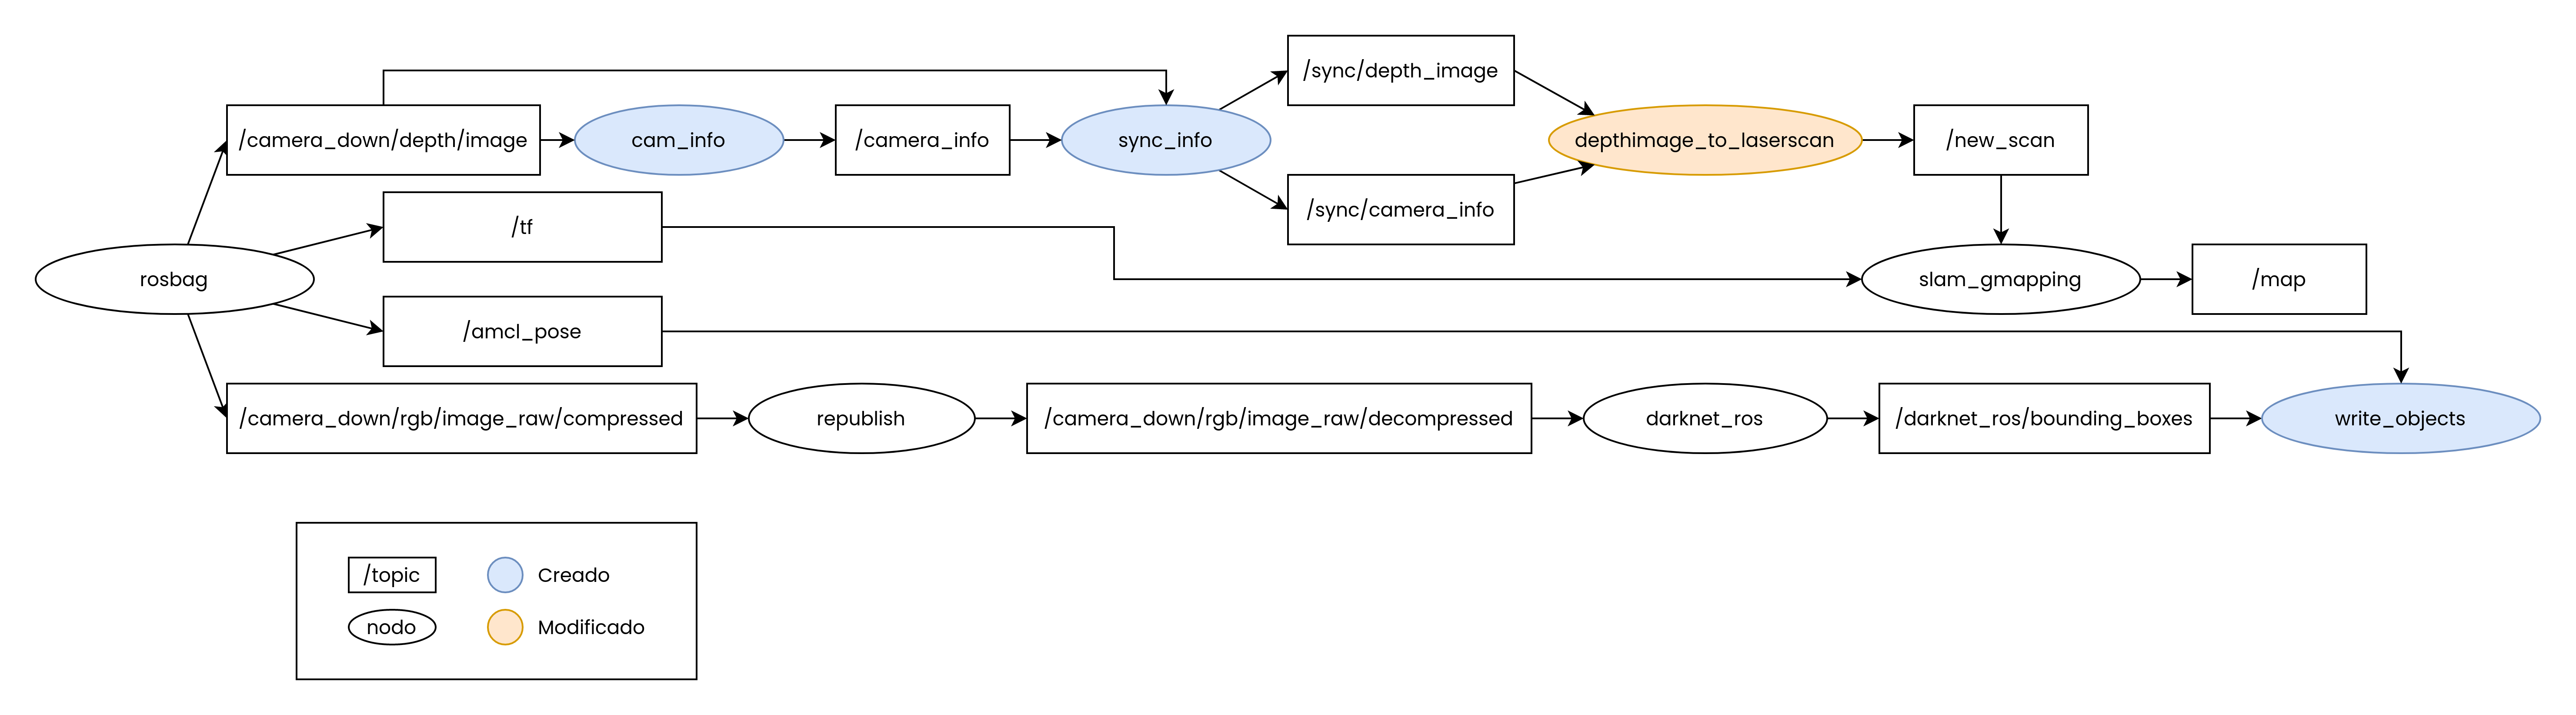
\includegraphics[width=\textwidth]{esquema_general.png}
	\end{center}
	\caption{Árbol de nodos y topics. Los nodos diseñados para este trabajo son de color azul. Los nodos de terceros cuyo código ha sido modificado son de color naranja. Los nodos descargados que no se han modificado son de color blanco}
	\label{fig:esq_general}
\end{figure}

A continuación se enumeran todos los nodos que se van a utilizar en este proyecto:

\begin{itemize}

	\item El nodo \texttt{cam\_info} es un nodo diseñado expresamente para este trabajo. Se encarga de recibir la cabecera de la imagen de profundidad para generar un mensaje con información de la cámara y publicarlo.
	\item El nodo \texttt{sync\_info} es otro de los que han sido diseñados para el proyecto. Su función es sincronizar los mensajes de la imagen de profundidad y de la información de la cámara.
	\item \texttt{depthimage\_to\_laserscan} es un nodo de un paquete homónimo diseñado por Chad Rocke \cite{di2ls} que se encarga, principalmente, de transformar una imagen de profundidad en un barrido láser en función de unos parámetros. Para implementar el nodo en este trabajo modificaremos algunos fragmentos de su código.
	\item El nodo \texttt{slam\_gmapping} es un nodo del paquete \texttt{gmapping} diseñado por Brian Gerkey \cite{gmapping}. Su función es la de obtener la localización del robot generando el mapa de ocupación.
	\item \texttt{republish} es un nodo que pertenece al paquete \texttt{image\_transport} diseñado por Patrick Mihelich \cite{republish}. Se encarga de descomprimir las imágenes de entrada y publicarlas en formato descomprimido.
	\item El nodo \texttt{darknet\_ros} es un nodo de un paquete con el mismo nombre diseñado por Marko Bjelonic \cite{darknet}. Implementa YOLO en ROS.
	\item El nodo \texttt{write\_objects} es un nodo diseñado para este proyecto con el fin de procesar los objetos detectados y escribirlos en un archivo de texto para su posterior análisis.
	

\end{itemize}


\section{Fuente de datos} \label{sec:datos}

La mejor manera de comprobar el correcto funcionamiento de todo el conjunto de nodos sería hacerlo directamente sobre el robot, con información real de sensores y del entorno. Sin embargo, debido a la dificultad que supondría utilizar este sistema sobre el robot, se decidió utilizar la herramienta que ROS pone a disposición precisamente para lidiar con este inconveniente: los rosbags.\\

Para este proyecto se va a utilizar un rosbag generado por uno de los robots del laboratorio de Automática de la Escuela Técnica Superior de Informática. Esta grabación recoge la información de la pose del robot (posición X e Y y el ángulo de orientación), los datos recogidos por una cámara RGB-D (color y profundidad), el barrido de un láser y otra información que típicamente se utiliza en los robots como el árbol de transformadas.\\

Sin embargo, pese a que este rosbag ha sido el utilizado para comprobar el funcionamiento del algoritmo diseñado, ha sido necesario hacer algunas modificaciones para que se pueda procesar la información correctamente.\\

Normalmente, cuando se utiliza una cámara RGBD en ROS, el paquete encargado de controlar la cámara envía tres tipos de mensajes pertenecientes al paquete sensor\_msgs. Estos mensajes son:

\begin{itemize}

	\item Imagen a color. Información de color de la imagen capturada con un mensaje de tipo Image. La mayoría de cámaras ofrece además la imagen rectificada, sin distorsiones.
	\item Imagen de profundidad. Información sobre la profundidad de la imagen capturada con un mensaje de tipo Image. Al igual que con la de color, también se ofrece la imagen rectificada.
	\item Parámetros de la cámara. Información sobre las propiedades de la cámara con un mensaje de tipo CameraInfo. Contiene datos sobre las propiedades de la imagen (ancho y alto) y parámetros de calibración de la cámara.

\end{itemize}

Debido a algunos problemas que se tuvieron durante la captura de los datos, este último topic no se ofrece en el rosbag, por lo que es necesario generarlo externo al rosbag. Para ello, se ha diseñado un nodo llamado \texttt{cam\_info} que se encarga de generar este mensaje que más tarde será utilizado por otros nodos.\\

\begin{figure}[h]
	\begin{center} 
		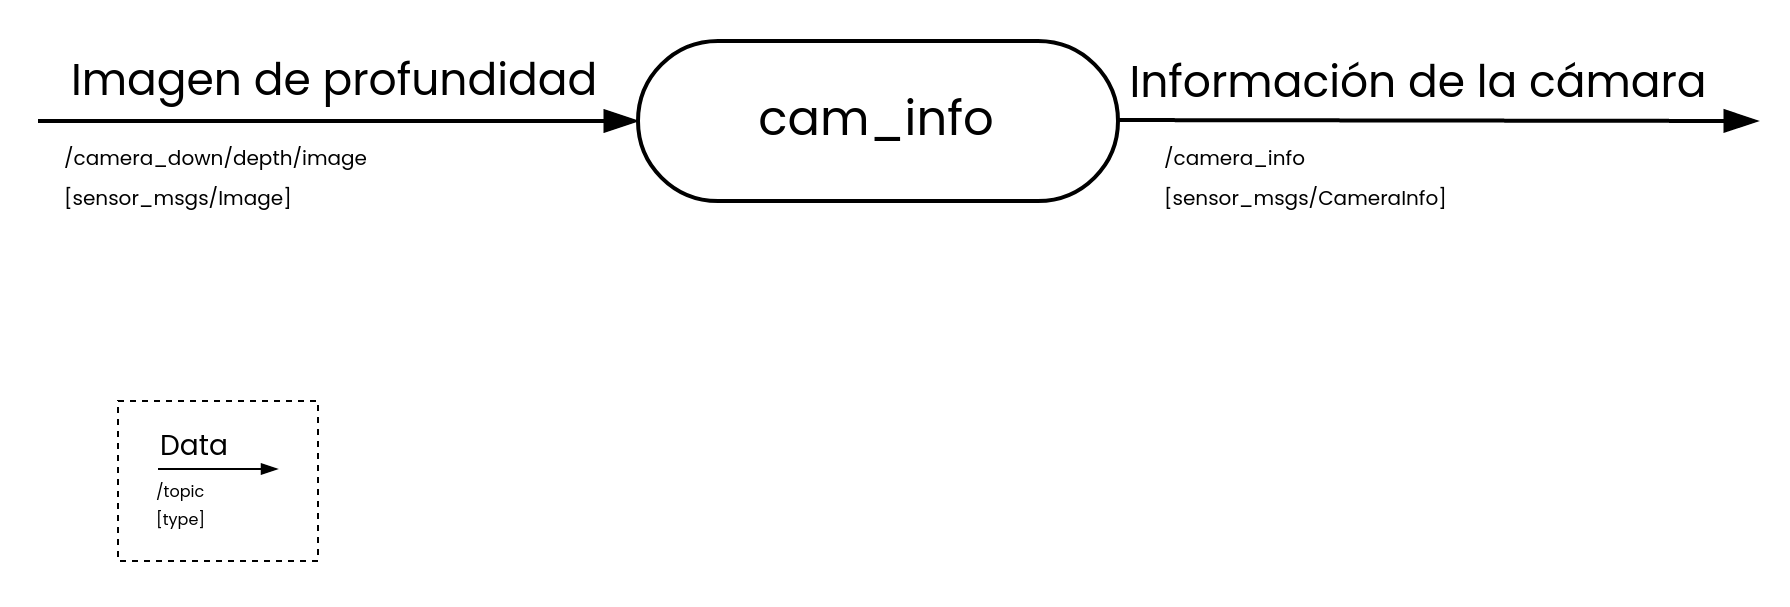
\includegraphics[width=\textwidth]{cam_info-diag.png}
	\end{center}
	\caption{Diagrama del nodo \texttt{cam\_info}. Recibe la imagen de profundidad y publica la información de la cámara}
	\label{fig:cam_info}
\end{figure}

Este nodo, programado en C++, recibe el mensaje de la imagen de profundidad ofrecido por el rosbag, copia su encabezado, crea el mensaje de tipo \texttt{sensor\_msgs/\-CameraInfo} con los parámetros de la cámara y lo envía por el topic \texttt{/camera\_info}.\\

Finalmente, una vez generado el mensaje con la información de los parámetros de la cámara, es necesario sincronizar estos topics para que puedan ser utilizados por otros nodos. Para ello se ha diseñado un nodo en Python llamado \texttt{sync\_info} que se sirve del paquete \texttt{message\_filter} para realizar este proceso. Se ha programado en Python porque resulta más fácil utilizar esta librería en este lenguaje que en C++.\\

\begin{figure}[h]
	\begin{center} 
		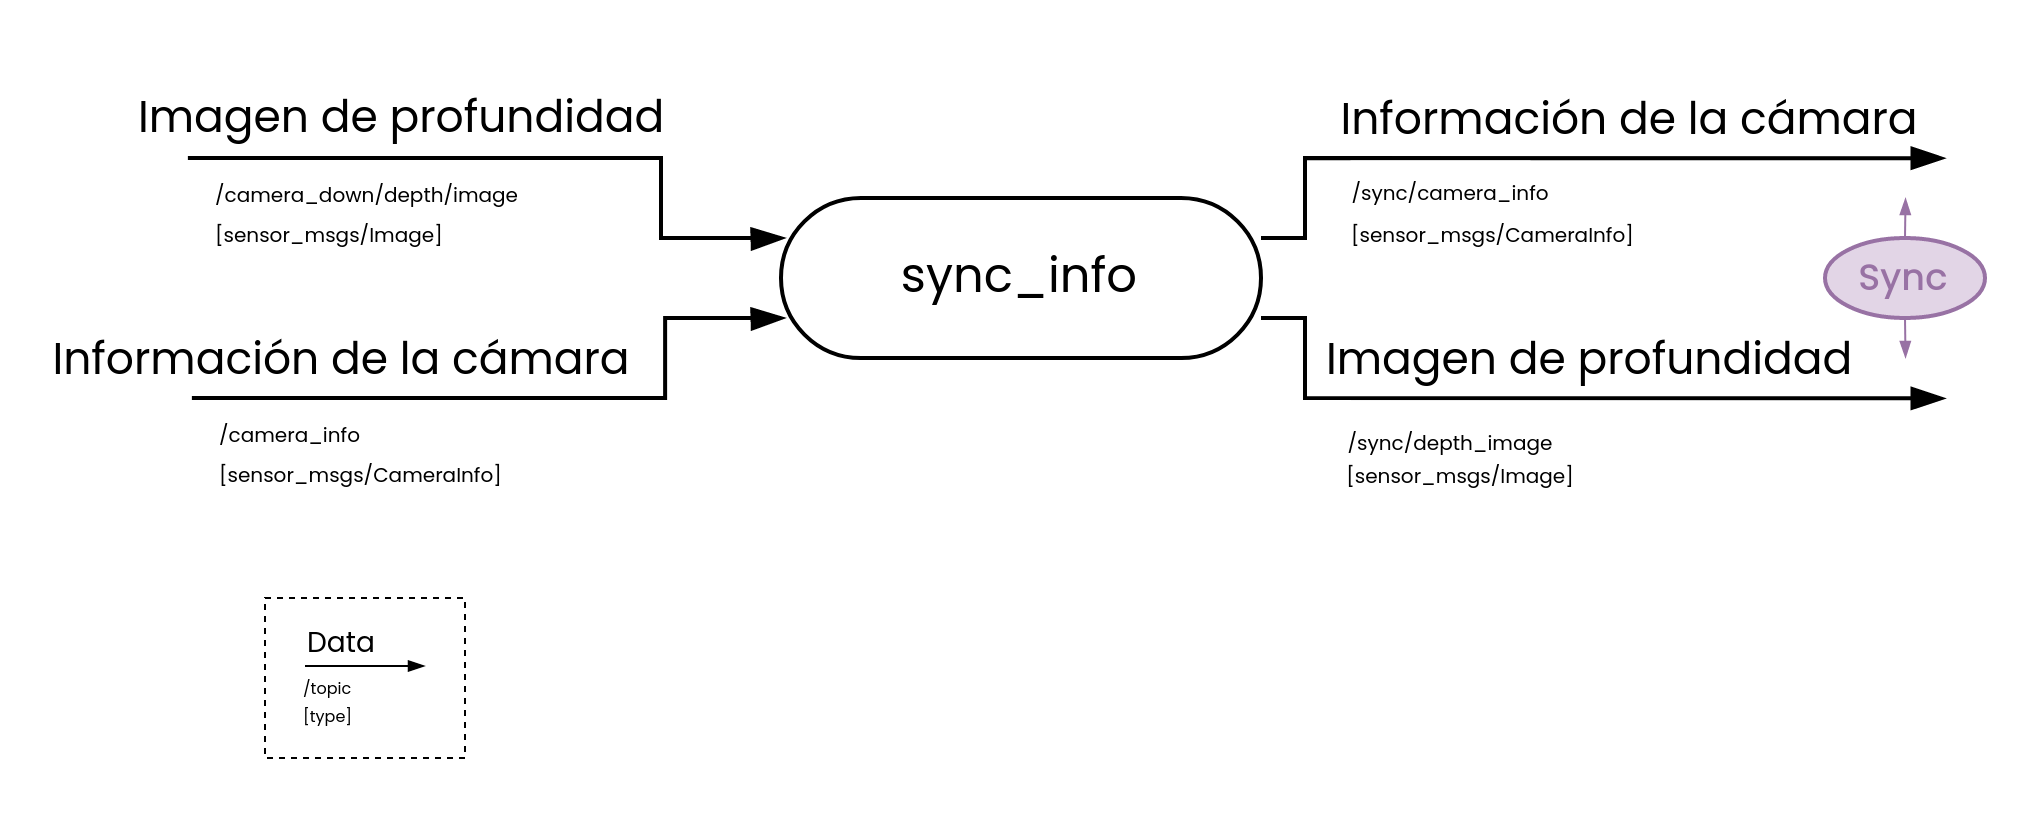
\includegraphics[width=\textwidth]{sync_info-diag.png}
	\end{center}
	\caption{Diagrama del nodo \texttt{sync\_info}. Recibe la imagen de profundidad y la información de la cámara y publica los mismo mensajes pero sincronizados}
	\label{fig:sync_info}
\end{figure}

\section{De imagen de profundidad a barrido láser} \label{depthimage_section}

Una vez se tiene toda la información ofrecida por el robot y la cámara correctamente sincronizada y configurada, es momento de realizar el procedimiento principal de este proyecto: transformar la imagen de profundidad obtenida mediante la cámara RGB-D en un barrido láser equivalente, cogiendo la distancias más alejadas captadas en la imagen. De esta forma, si tenemos varios objetos delante de una pared, con el algoritmo diseñado no se tendrán en cuenta estos objetos y se seleccionarán siempre las distancias menos restrictivas para generar el láser. Es necesario generar un láser artificial porque los algoritmos que se utilizan para generar el mapa de ocupación utilizan este tipo de datos.\\

El algoritmo utilizado está basado en el paquete de ROS \texttt{depthimage\-\_to\_\-laserscan}. Este paquete se encarga de transformar una imagen de profundidad en un barrido láser a partir de los parámetros de la cámara y de una serie de parámetros de entrada configurables. Los parámetros se muestran en el cuadro \ref{tab:param_depthimage}.

\begin{table}[H]
\begin{center}
\begin{tabular}{| w{c}{3cm} | w{c}{3cm} | m{7.5cm} |}
	\hline
	Parametro & Valor por defecto & Descripción \\ \hline
	\texttt{scan\_height} & 1 & Establece la cantidad de filas que se quieren procesar para generar el láser \\ \hline
	\texttt{scan\_time} & 0.033 (30FPS) & Establece el tiempo de actualización entre escaneos \\ \hline
	\texttt{range\_min} & 0.45 metros & Rango de distancia mínima. Valores medidos menores que este valor se tomarán como -Inf \\ \hline
	\texttt{range\_min} & 10 metros & Rango de distancia máxima. Valores medidos menores que este valor se tomarán como +Inf \\ \hline
	\texttt{output\_frame\_id} & \texttt{laser} & Establece el id del eje de coordenadas (frame) de salida. Se indica el id del frame del láser \\ \hline
\end{tabular}
\caption{Formato del archivo CSV generado}
\label{tab:param_depthimage}
\end{center}
\end{table} 

Este nodo primeramente recibe la imagen de profundidad y la información de la cámara. Se recuerda que estos mensajes los debe recibir a la vez y por eso requería de la sincronización. Una vez recibidos estos mensajes, evalúa la codificación de la imagen. Si la codificación es correcta (admite codificación 16UC1 o 32FC1)\footnote{El paquete \texttt{sensor\_msgs} prove de multitud de codificaciones para las imaǵenes. Este es un parámetro de la imagen y viene dado por una cadena de caracteres \cite{enc}. El paquete \texttt{depthimage\_to\_laserscan} solo admite las dos codificaciones comentadas.}, procede a convertir la imagen de profundidad a un mensaje de tipo LaserScan. El formato de un mensaje de tipo \texttt{LaserScan} se expone en el cuadro \ref{tab:laserscan_msg}.\\

\begin{table}[H]
\begin{center}
\begin{tabular}{| w{c}{4cm} | m{6.5cm} |}
	\hline
	Parámetro & Descripción \\ \hline
	\texttt{header} & Encabezado del mensaje. Propiedad que tienen todos los mensajes \\ \hline
	\texttt{angle\_min} & Ángulo mínimo que abarca el láser en radianes \\ \hline
	\texttt{angle\_max} & Ángulo máximo en radianes \\ \hline
	\texttt{angle\_increment} & Ángulo entre medidas en radianes \\ \hline
	\texttt{time\_increment} & Tiempo entre medidas en segundos \\ \hline
	\texttt{scan\_time} & Tiempo entre escaneos en segundos \\ \hline
	\texttt{range\_min} & Rango mínimo del sensor en metros \\ \hline
	\texttt{range\_max} & Rango máximo del sensor en metros \\ \hline
	\texttt{ranges} & Vector con las medidas tomadas en metros \\ \hline
	\texttt{intensities} & Vector con las intensidades de las medidas. Se tomará como un array vacío porque no es necesario \\ \hline
\end{tabular}
\caption{Formato de un mensaje de tipo \texttt{LaserScan}}
\label{tab:laserscan_msg}
\end{center}
\end{table} 

El algoritmo se encarga de analizar tantas filas como se establezcan en el parámetro \texttt{scan\_height} del nodo \texttt{depthimage\_to\_laserscan} y transformar la distancia dada por la imagen de profundidad en una distancia real al sensor. Una vez transformada, se compara con la distancia de las otras filas medidas en la misma columna y, si la distancia es mayor, se añade al vector ranges. Una vez completado el análisis de todas las filas de la imagen, se publica el mensaje generado de tipo \texttt{sensor\_msgs/LaserScan} en el topic \texttt{/new\_scan}.\\

\section{Generación del mapa de ocupación} \label{mapa_ocup}

Una vez obtenido el láser artificial a partir de la imagen de profundidad, es momento de generar el mapa o rejilla de ocupación. Para este procedimiento se utilizará el paquete \texttt{gmapping}.\\

Este paquete ofrece un sistema de Localización y Mapeado Simultáneo o SLAM (del inglés, \textit{Simultaneous Location and Mapping}) a través de un nodo llamado \texttt{slam\_gmapping}. Este nodo recibe el láser artificial (por el topic \texttt{/new\_scan}) y el árbol de transformadas (por el topic \texttt{/tf}).\\

Al lanzar este nodo, es posible establecer multitud de parámetros que determinan el modo de operación. Entre otros, los parámetros que se tendrán en cuenta para ajustar el resultado acorde al objetivo son:

\begin{itemize}

	\item \texttt{linearUpdate}. El nodo procesará un escaneo cada vez que se alcance la distancia lineal determinada por este parámetro. Su valor por defecto es $1.0$. El valor óptimo encontrado tras múltiples pruebas es $0.3$.
	\item \texttt{angularUpdate}. Determina el incremento de ángulo por el cuál el robot procesará otro escaneo. Su valor por defecto es $0.5$. El valor óptimo es $0.7$.
	\item \texttt{temporalUpdate}. Establece cada cuánto se procesa un nuevo escaneo. Su valor por defecto y óptimo es $3.0$.

\end{itemize}

Como se comenta en el listado de parámetros, tienen unos valores por defecto que se han ido modificando para obtener un mapa con más fiable. Esto se comentará más en profundidad en la sección de resultados.\\

El nodo \texttt{slam\_gmapping} envía por el topic \texttt{/map} mensajes de tipo \texttt{nav\_msgs\-/OccupancyGrid} con información sobre el mapa de forma que, tras finalizar la reproducción del rosbag, el último mensaje enviado por este topic contendrá el mapa completo que se ha generado. Para guardarlo en un formato con el que poder trabajar, se utiliza el nodo \texttt{map\_saver} del paquete \texttt{map\_server}, diseñado por Brian Gerkey y Tony Pratkanis. Simplemente se lanza el nodo dándole como parámetro el nombre con el que se va a guardar el mapa. Finalmente se obtienen dos archivos: un \texttt{.yaml}, para la configuración, y otro en formato \texttt{.pgm} para la imagen.\\

\section{Detección de objetos}

Paralelamente, se ha diseñado un sistema capaz de interpretar la imagen a color proporcionada por el sensor RGBD para detectar los objetos y tener un registro de los mismos. Este sistema, en principio, se puede lanzar simultáneamente junto con el sistema de generación de mapas de ocupación, sin embargo, debido a la potencia necesaria para ejecutar la red neuronal por GPU, resulta tedioso e incluso problemático con algunos ordenadores. Es por ello que se ha diseñado para que pueda ser lanzado de forma asíncrona con respecto al otro sistema.\\

\subsection{Descompresión de la imagen de color}

En muchas ocasiones, los paquetes de ROS que sirven para utilizar determinadas marcas de sensores RGBD proporcionan las imágenes en un formato comprimido para ahorrar potencia. Con el rosbag que se ha utilizado como fuente de datos ocurre lo mismo, por lo que es necesario un proceso de descompresión.\\

Para este procedimiento, se ha utilizado un nodo llamado \texttt{republish} del paquete \texttt{image\_transport}. Este nodo se recibe un mensaje en formato \texttt{sensor\_msgs/\-Compressed\-Image} y lo convierte en un mensaje de tipo \texttt{sensor\_msgs/Image} para publicarlo.\\

\subsection{Ejecución de YOLO}

Una vez la imagen está descomprimida, ya puede ser recibida por la red neuronal. Este nodo recibe la imagen de color en formato \texttt{sensor\_msgs/Image} y publica en tres topics:

\begin{itemize}

	\item \texttt{object\_detector}. Mensaje de tipo \texttt{std\_msgs/Int8} que indica el número de objetos detectados.
	\item \texttt{bounding\_boxes}. Mensaje de tipo \texttt{darknet\_ros\_msgs/BoundingBoxes} que representa un array que proprociona información sobre la posición y el tamaño de los bounding boxes en píxeles.
	\item \texttt{detection\_image}. Mensaje de tipo \texttt{sensor\_msgs/Image} que ofrece las bounding boxes detectadas sobre la imagen a color que ha sido procesada.
	
\end{itemize}

Las bounding boxes son unas ``cajas'' que señalizan al elemento detectado. Un mensaje de tipo \texttt{darknet\_ros\_msgs/BoundingBoxes} es un array de elementos con formato \texttt{darknet\_ros\_msgs/BoundingBox}.\\

Además, este nodo ofrece una salida en la terminal indicando los frames por segundo (FPS) a los que se está ejecutando y un listado de los objetos encontrados junto con sus probabilidades, como se muestra en la figura \ref{fig:yolo_funcionando}. YOLO tiene un umbral de probabilidad establecido por defecto en $0.7$ para aceptar una detección como válida o no. \\

\begin{figure}[h]
	\begin{center} 
		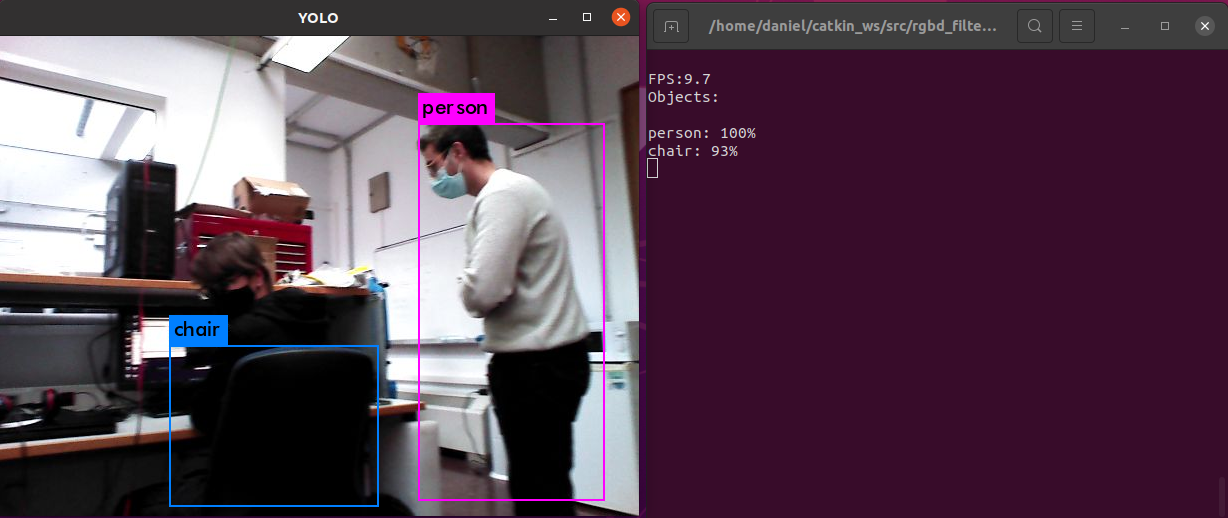
\includegraphics[width=\textwidth]{yolo_funcionando.png}
	\end{center}
	\caption{Salida en la terminal del nodo \texttt{darknet\_ros}. En la parte izquierda se muestran las bounding boxes sobre la imagen a color. A la derecha, en la terminal, se muestran los FPS actuales y los objetos y sus probabilidades}
	\label{fig:yolo_funcionando}
\end{figure}

\section{Procesamiento de los objetos detectados}

Como se ha comentado, a partir del nodo que implementa YOLO obtenemos un array de bounding boxes con información sobre la posición y el tamaño en píxeles. Para el desarrollo de este proyecto se ha visto conveniente procesar esa información para realizar un posterior estudio de los objetos que han sido detectados y analizar la fiabilidad de la red neuronal así como la calidad de los datos proporcionado por el rosbag.\\

Para este procesamiento se ha diseñado un nodo llamado \texttt{write\_objects} que se encarga de recibir los mensajes que se publican en \texttt{/darknet\_ros/bounding\_boxes} y en \texttt{/amcl\_pose} para generar un archivo CSV donde cada fila representa la información con el formato mostrado en el cuadro \ref{tab:formato}. Cada columna utilizará el delimitador de punto y coma (`` ; '').\\

\begin{table}[H]
\begin{center}
\begin{tabular}{| c | c | c | c | c |}
	\hline
	Objetos & Probs & Posición & Orientación & Tiempo \\ \hline
	obj1:obj2:...:objN & prob1:prob2:...:probN & pX:pY:pZ & oW:oX:oY:oZ & (seg) \\ \hline

\end{tabular}
\caption{Formato del archivo CSV generado}
\label{tab:formato}
\end{center}
\end{table} 

Toda esta información es obtenida a partir del formato de los mensajes de las bounding boxes y de la pose. Para las bounding boxes es necesario acceder a cada una de ellas y obtener sus propiedades \texttt{Class} y \texttt{probability}. Para la pose es necesario acceder a su propiedades \texttt{pose.pose.position} y \texttt{pose.pose.orientation}. El formato del mensaje de una bounding box se representa en el cuadro \ref{tab:boundingbox_msg}.\\

\begin{table}[H]
\begin{center}
\begin{tabular}{| w{c}{4cm} | m{8cm} |}
	\hline
	Parámetro & Descripción \\ \hline
	\texttt{probability} & Probabilidad de que el elemento detectado sea realmente de la clase que se le atribuye \\ \hline
	\texttt{xmin} & Coordenada X mínima de la bounding box en píxeles \\ \hline
	\texttt{ymin} & Coordenada Y mínima de la bounding box en píxeles \\ \hline
	\texttt{xmax} & Coordenada X máxima de la bounding box en píxeles \\ \hline
	\texttt{ymax} & Coordenada Y máxima de la bounding box en píxeles \\ \hline
	\texttt{id} & Identificador único para cada bounding box \\ \hline
	\texttt{Class} & Clase o etiqueta del elemento detectado \\ \hline
\end{tabular}
\caption{Formato de un mensaje de tipo \texttt{BoundingBox}}
\label{tab:boundingbox_msg}
\end{center}
\end{table} 


\section{Análisis de los objetos detectados}

Una vez obtenido el registro de los objetos en formato CSV es posible procesar esta información para realizar un análisis de la red y del entorno. Para ello se utilizará el entorno de programación en Python de \textit{Google Colab}, junto con las librerías \textit{Pandas} y \textit{Matplotlib}.La información sobre las gráficas y los resultados obtenidos se exponen en el capítulo siguiente.\\

\chapter{Resultados obtenidos} \label{chapter.resultados}

En este capítulo se mostrarán los resultados que se han obtenido tras implementar el sistema. Primeramente se expondrá el mapa generado con la imagen de profundidad y los mapas obtenidos utilizando diferentes parámetros. Luego se hará una comparativa con el resultado obtenido a partir del láser 2D incorporado en el robot. En una segunda parte se mostrarán algunas gráficas realizadas con el registro de objetos detectados y se expondrán los posibles errores de la red neuronal en el proceso de la detección.\\

\section{Mapa generado a partir de la imagen de profundidad}

En la figura \ref{fig:res_mapas} se muestra el resultado de generar el mapa a partir del láser 2D (izquierda) y a partir de la imagen de profundidad captada por el sensor RGBD (derecha).\\

\begin{figure}[h]
 \centering
  \subfloat[Generado con láser 2D]{
    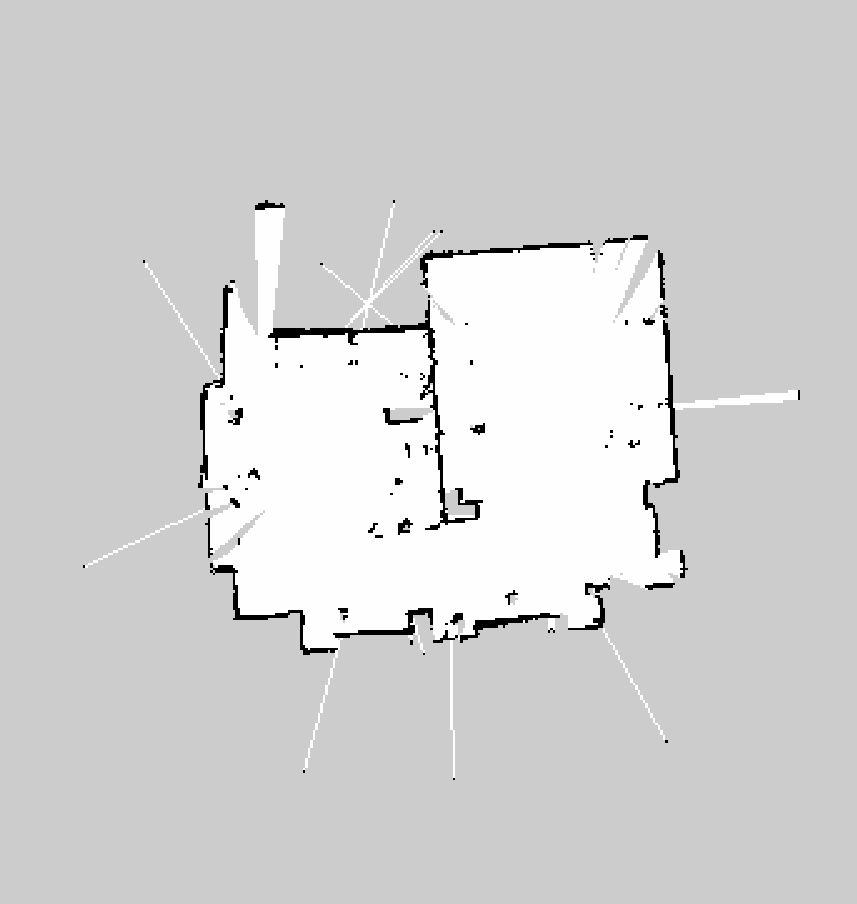
\includegraphics[width=0.4\textwidth]{mapa_laser.png}}
  \subfloat[Generado con sensor RGBD]{
    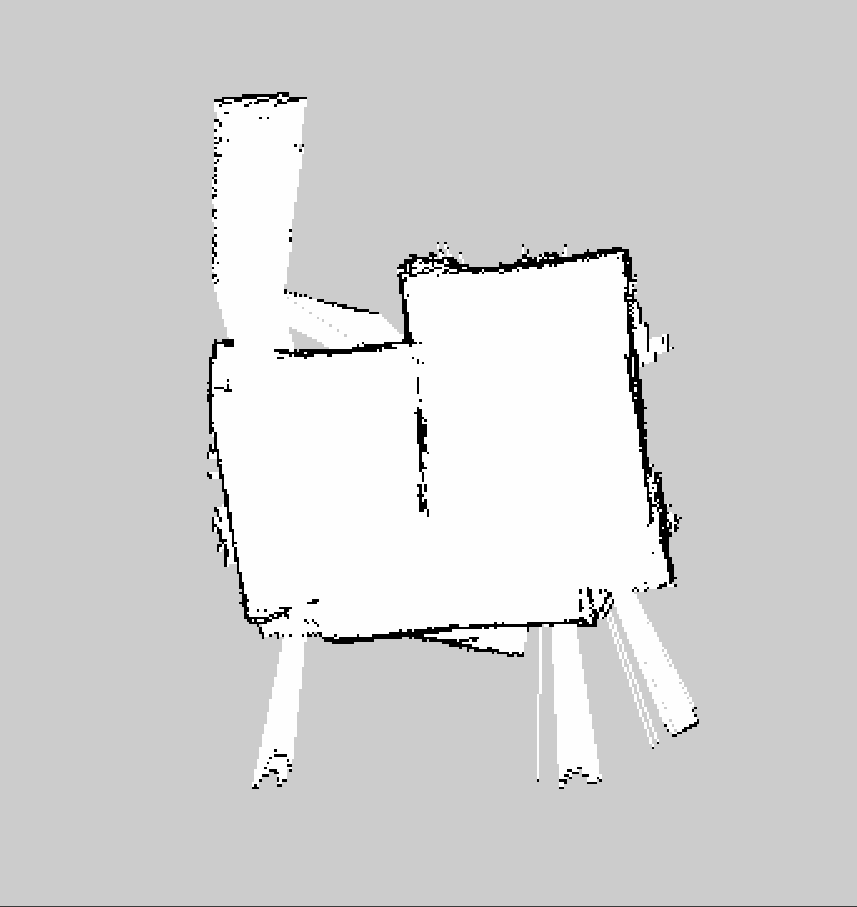
\includegraphics[width=0.4\textwidth]{mapa_corregido_bien.png}}
 \caption{Mapas generados con láser 2D (a) y con sensor RGBD (b). Se puede observan la diferencia de rectitud en las líneas exteriores (problema) así como lo poco ruidoso que resulta el interior (virtud)}
 \label{fig:res_mapas}
\end{figure}

En el mapa generado con el láser se pueden ver los entrantes y salientes se forman debido a la presencia de mobiliario delante de las paredes que impide obtener una medida real de la estructura. Además, en zonas interiores existen muchos grupos pequeños de celdas ocupadas causadas por la presencia de patas de mesas, sillas y otros elementos de menor tamaño. Sin olvidar que la grabación cuenta con la presencia de personas que modifican su posición, complicando aún más la generación del mapa.\\

Con el mapa obtenido gracias al procesamiento de la imagen de profundidad, se puede comprobar como los elementos situdos entre el sensor y las paredes no se tienen en cuenta, quedando el interior del mapa totalmente ``limpio''. Además, las zonas donde se sitúa el mobiliario quedan mucho más suavizadas, mostrándose únicamente la pared stuada tras el mismo. En la figura \ref{fig:comp} se muestran los dos mapas superpuestos para poder ver mejor la diferencia entre sendos mapas.\\

Pese a que mejora al láser en muchos aspectos, el mapa generado con la cámara tiene numerosos problemas. Como se puede observar, las paredes no son totalmente rectas sino que tienen curvatura, lo que provoca que las esquinas no formen 90º. Incluso hay paredes, como la que está situada más a la izquierda, que parecen desviarse con respecto al mapa global.\\

\begin{figure}[h]
	\begin{center} 
		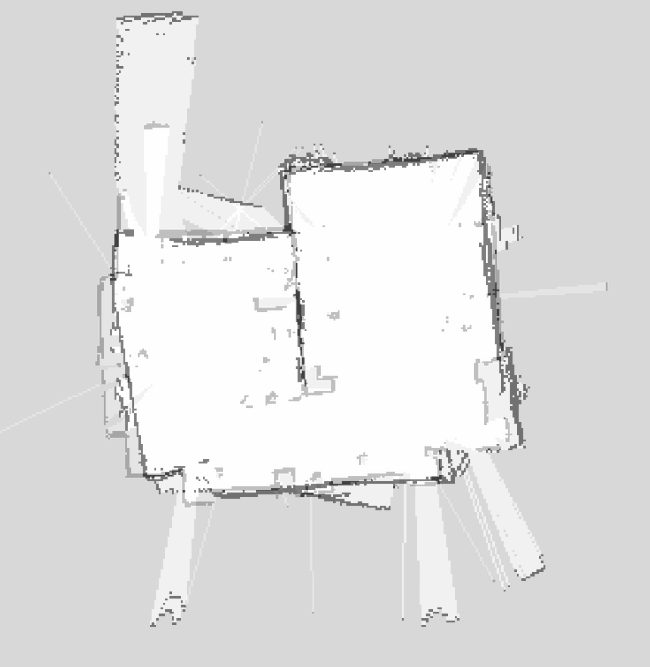
\includegraphics[width=0.5\textwidth]{comp.png}
	\end{center}
	\caption{Superposición de los dos mapas. Los objetos no estructurales se han eliminado correctamente}
	\label{fig:comp}
\end{figure}

Estas curvaturas obtenidas en la medición puede ser causada por la calibración intrínseca de la cámara. Es posible que algunos parámetros de la cámara no estén correctamente determinados o incluso que la transformada entre la base del robot y la cámara no esté correctamente establecida. Por la curvatura en las esquinas se intuye que la causa más probable sea una mala calibración de los parámetros de distorsión de la cámara.\\

Este resultado ya se podía percibir observando el láser generado a partir del sensor RGBD en comparación con el del láser 2D durante el proceso de construcción del mapa.\\

\subsection{Generación del láser artificial}

Como se ha comentado previamente, el láser que se genera a partir de la imagen de profundidad tiene unas curvaturas que ya se podían percibir claramente durante el proceso de generación del mapa. En muchas ocasiones, el láser artifical generado no se superpone con el láser real en las situaciones en las que debería hacerlo, como las de las figuras \ref{fig:m1} y \ref{fig:m2}.\\

En otras muchas ocasiones, como en las de las figuras \ref{fig:m3} e \ref{fig:m4}, se puede ver como el procesamiento realiza correctamente su función, cumpliendo el objetivo inicialmente establecido de ``eliminar'' los objetos frente a las paredes.\\

\begin{figure}[H]
	\begin{center} 
		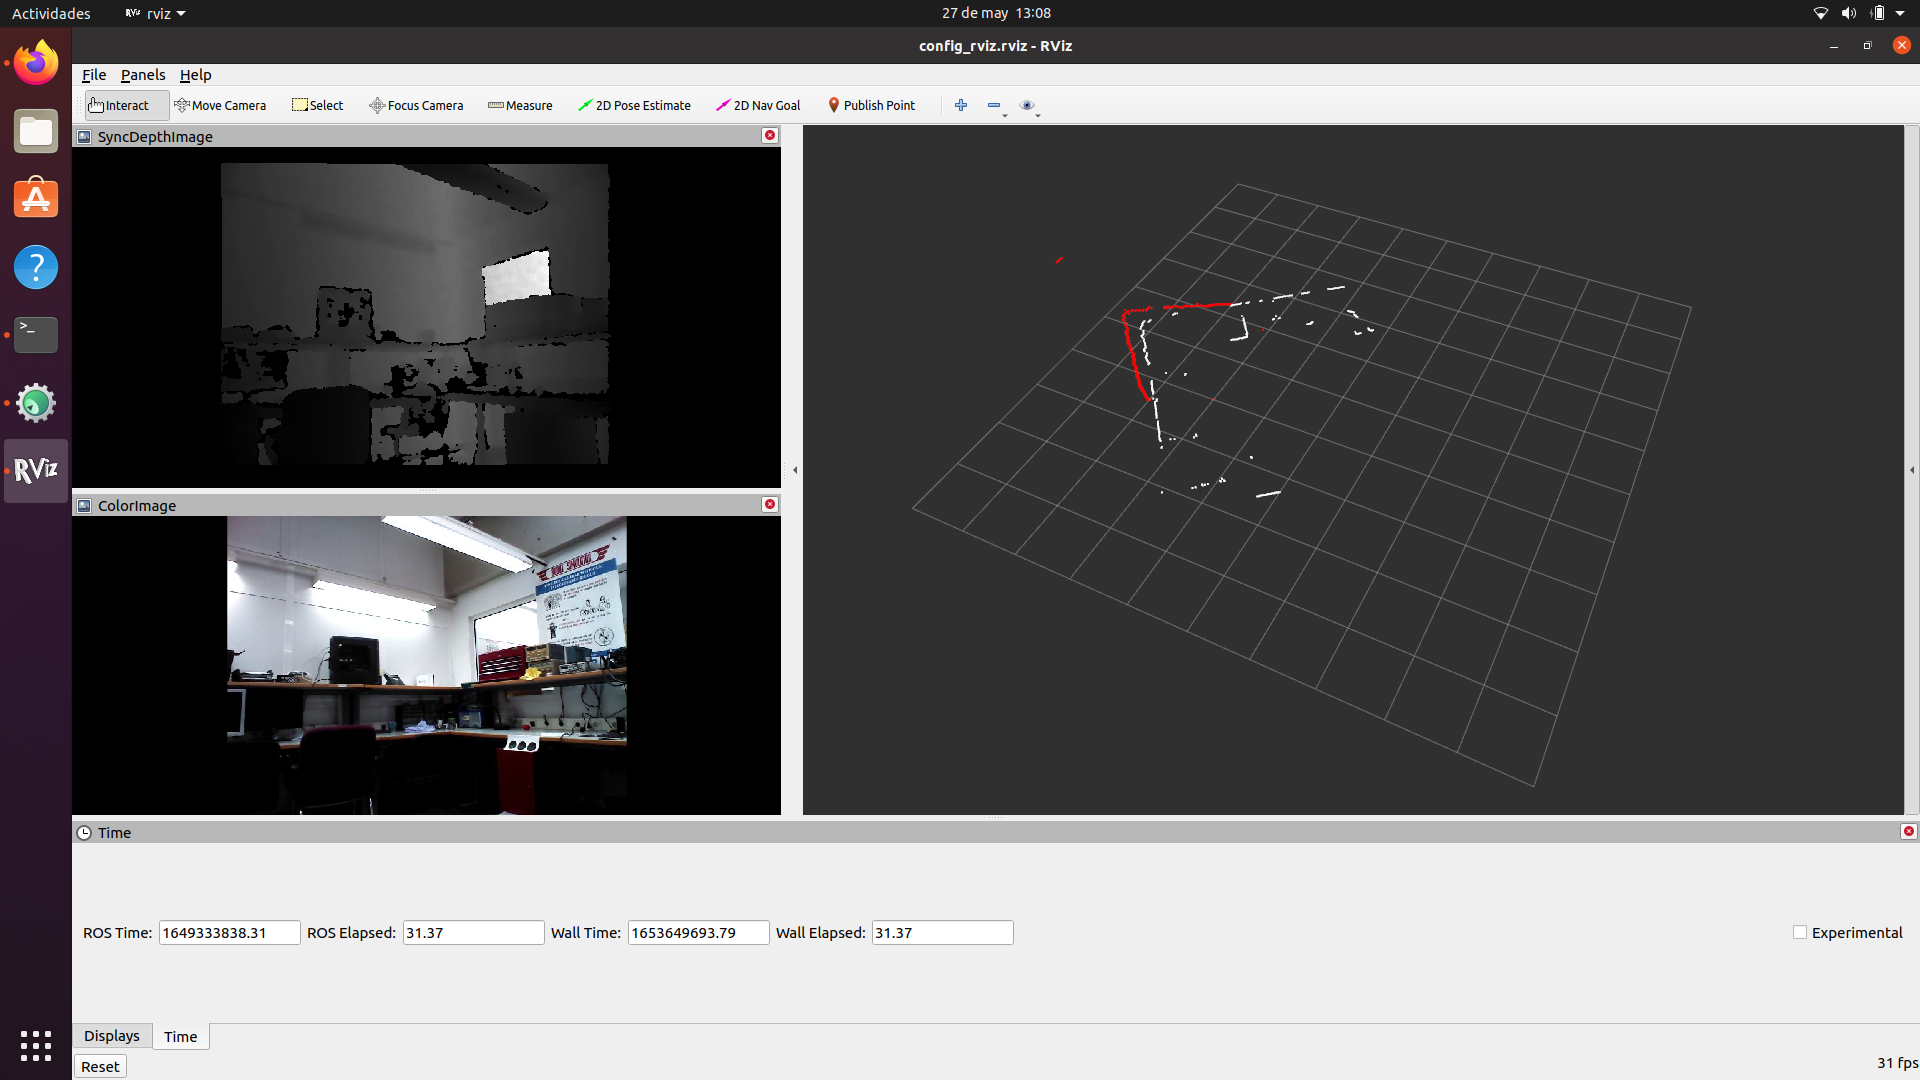
\includegraphics[width=\textwidth]{m1.png}
	\end{center}
	\caption{Muestra de medida 1: diferencia entre las medidas del láser real (blancas) y del láser artificial (rojas)}
	\label{fig:m1}
\end{figure}

\begin{figure}[H]
	\begin{center} 
		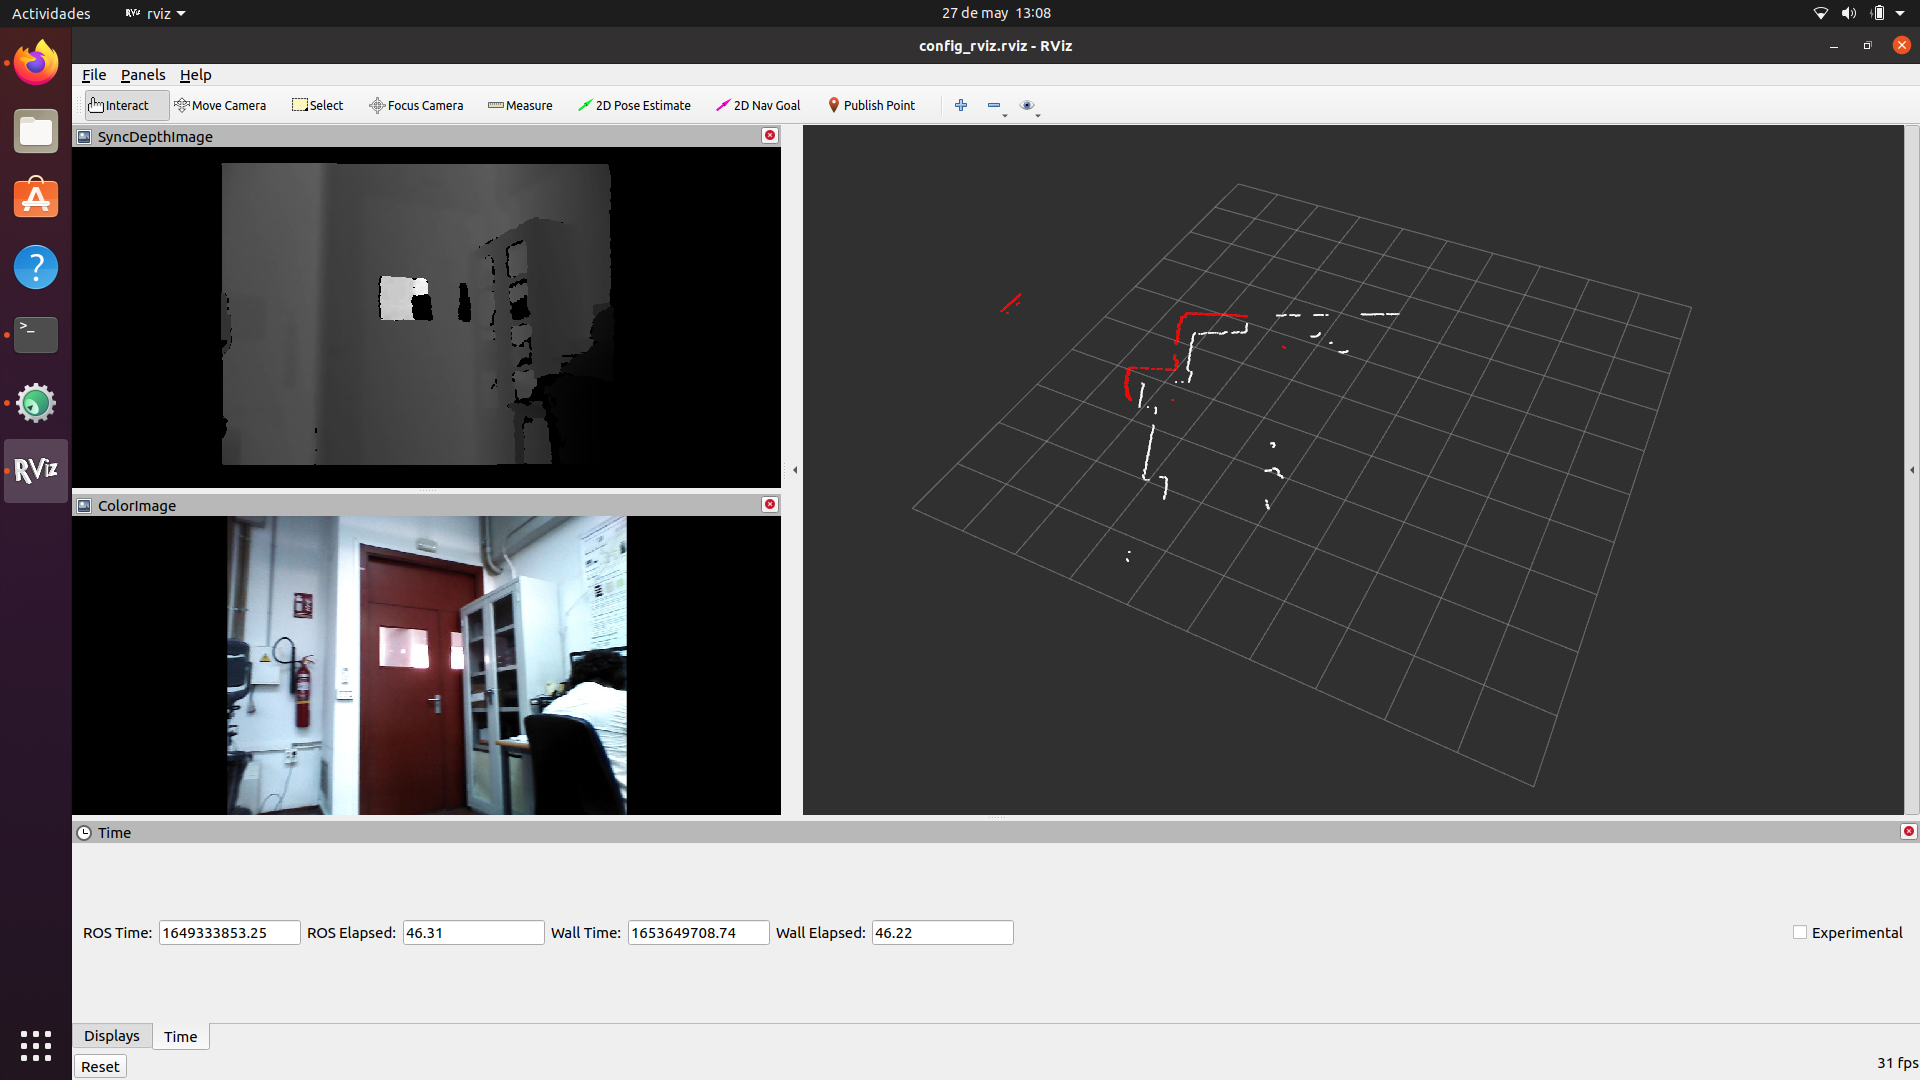
\includegraphics[width=\textwidth]{m2.png}
	\end{center}
	\caption{Muestra de medida 2: diferencia entre las medidas del láser real (blancas) y del láser artificial (rojas)}
	\label{fig:m2}
\end{figure}

\begin{figure}[H]
	\begin{center} 
		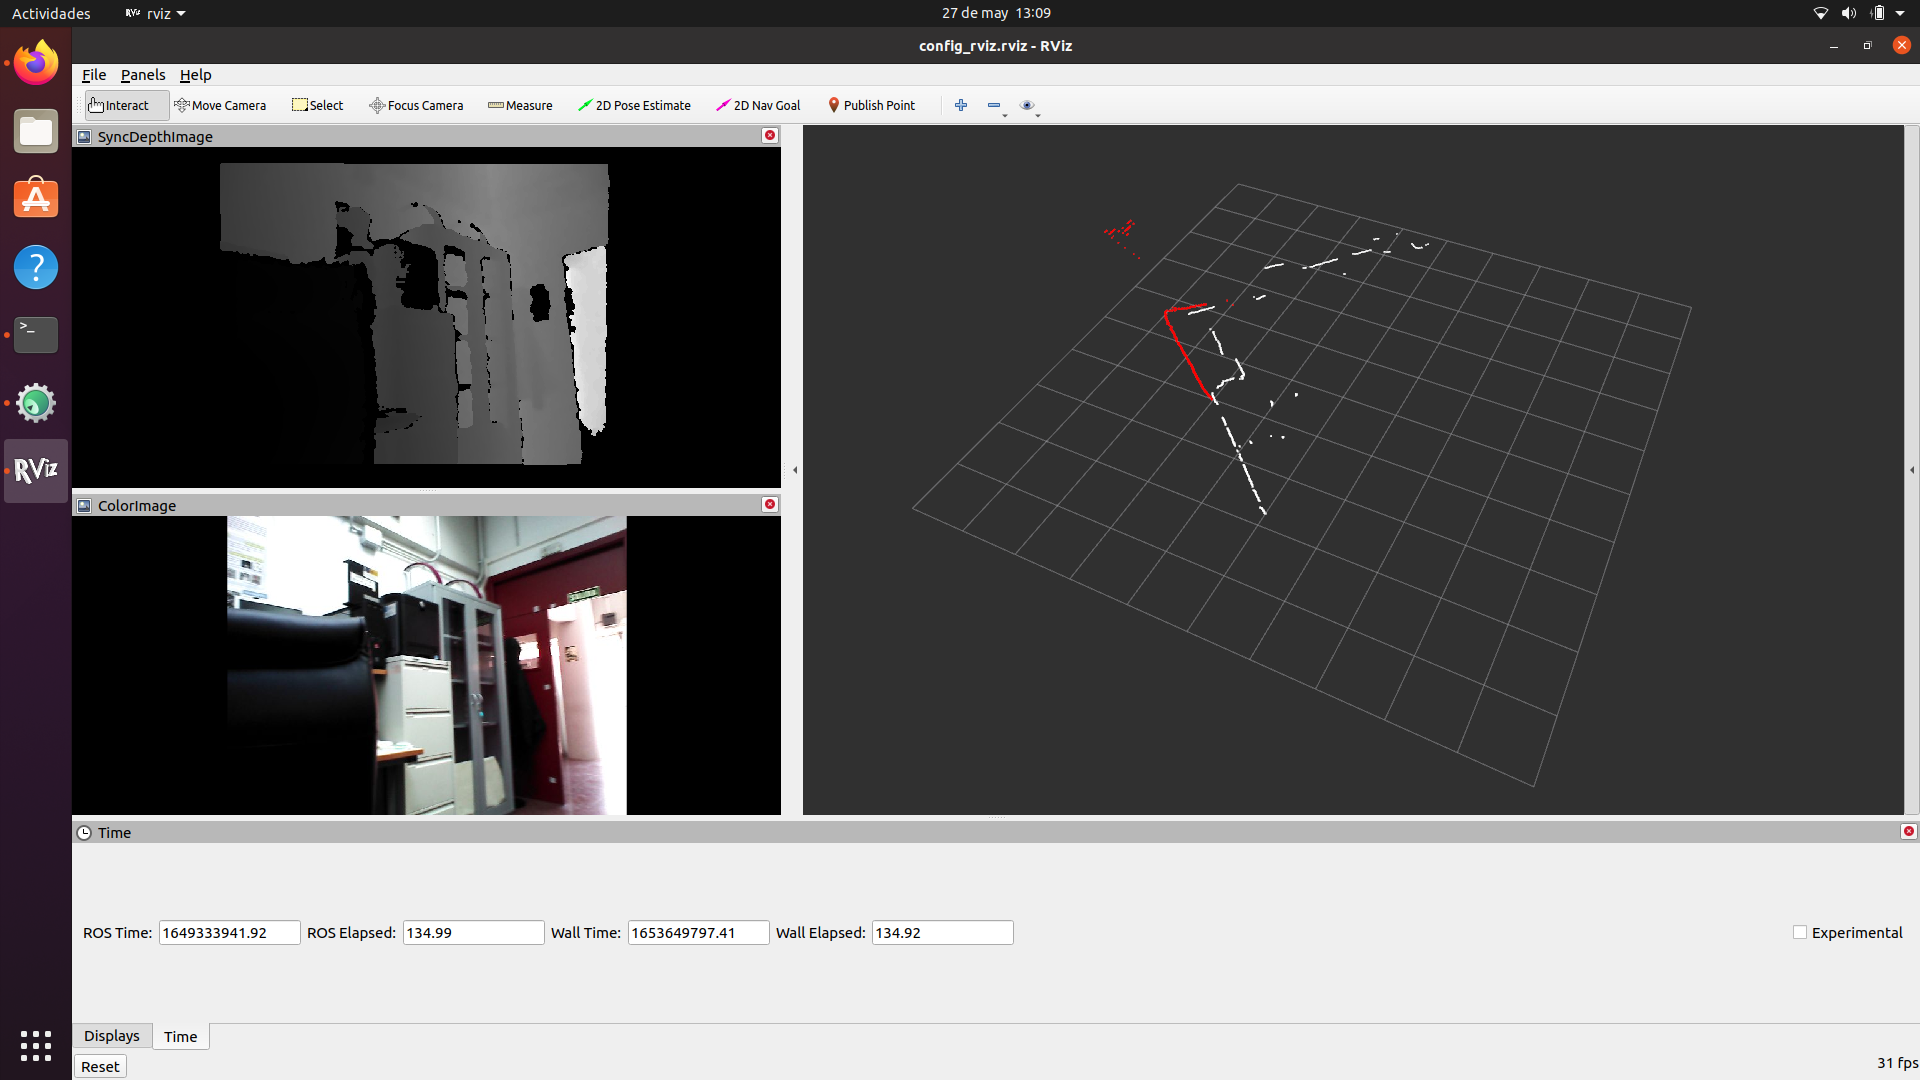
\includegraphics[width=\textwidth]{m3.png}
	\end{center}
	\caption{Muestra de medida 3: diferencia entre las medidas del láser real (blancas) y del láser artificial (rojas)}
	\label{fig:m3}
\end{figure}

\begin{figure}[H]
	\begin{center} 
		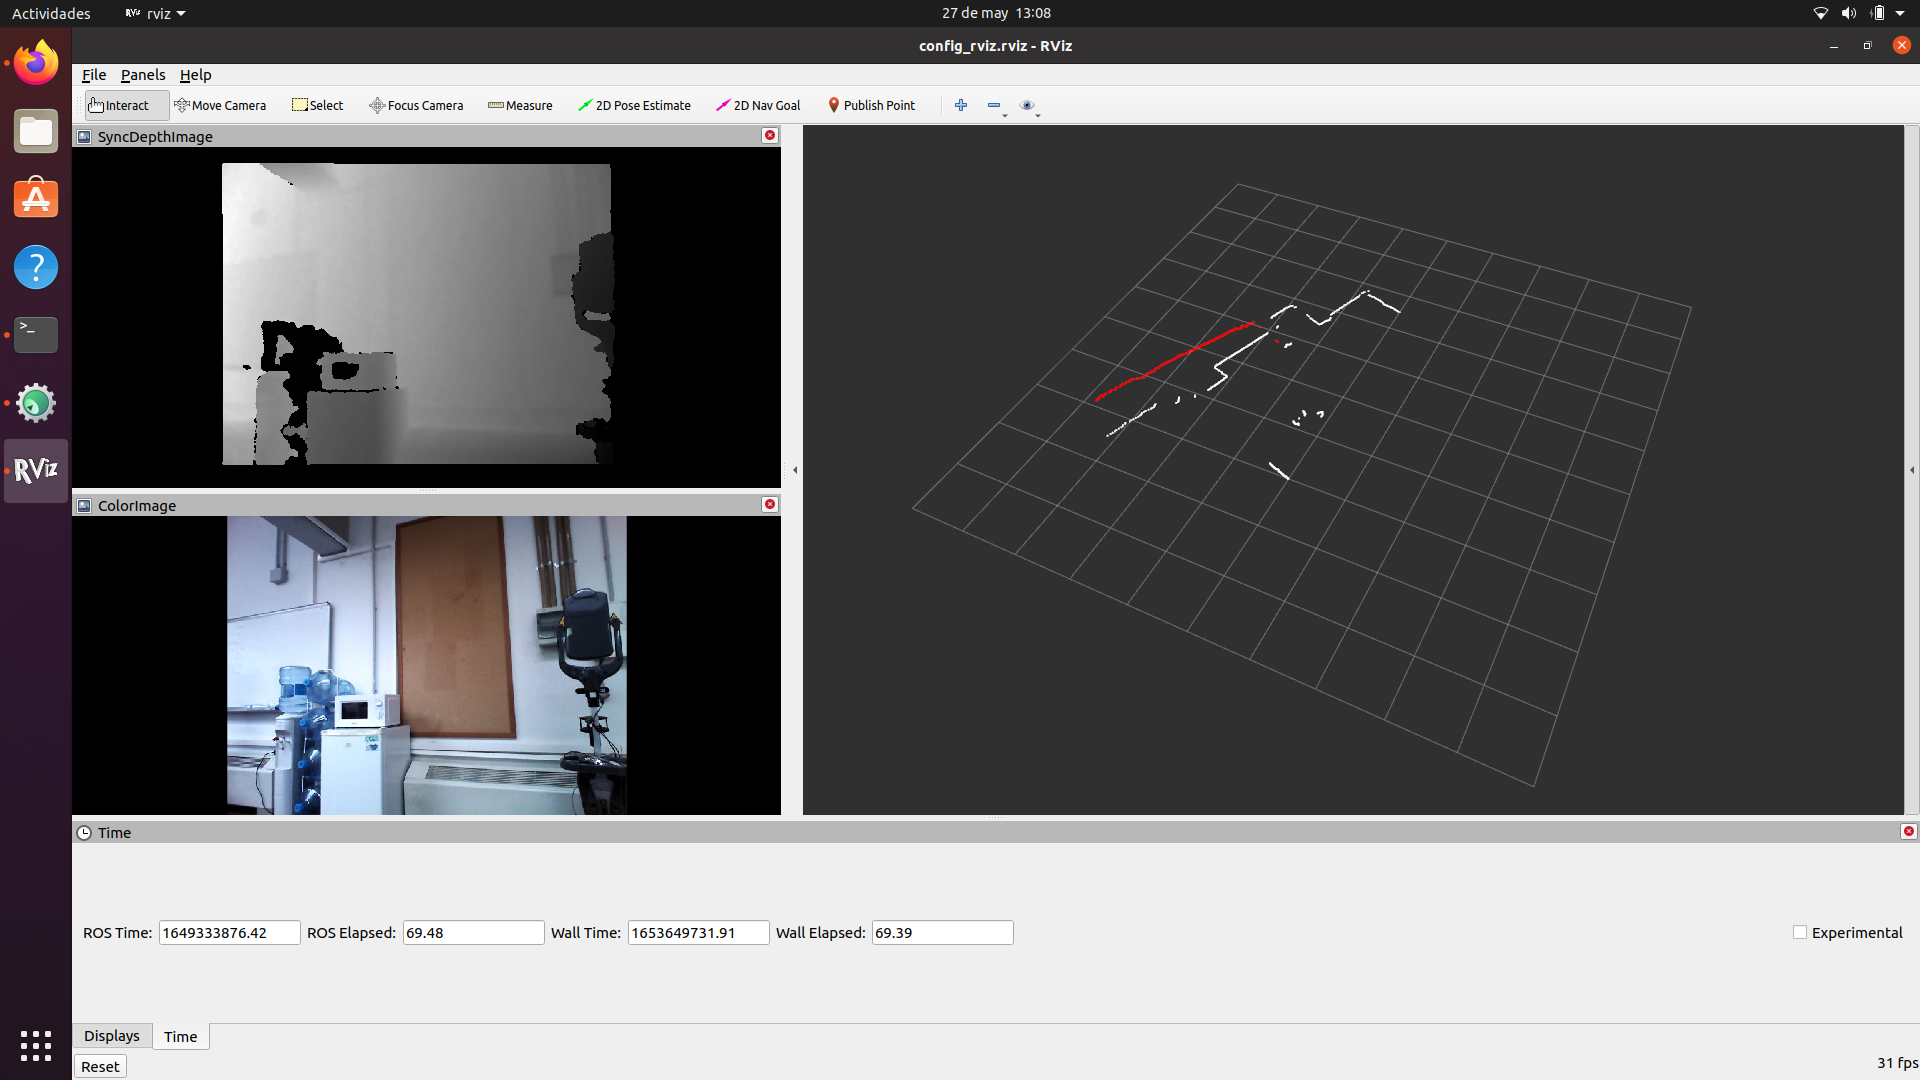
\includegraphics[width=\textwidth]{m4.png}
	\end{center}
	\caption{Muestra de medida 4: diferencia entre las medidas del láser real (blancas) y del láser artificial (rojas)}
	\label{fig:m4}
\end{figure}

\subsection{Modificación de parámetros por defecto}

Como se comentó en la sección \ref{mapa_ocup}, el nodo \texttt{slam\_gmapping} tiene una serie de parámetros que permiten ajustar cada cuántos metros, ángulos o segundos se procesa la información del láser.\\

Tras una primera ejecución del procedimiento diseñado, el resultado obtenido no fue el esperado. Es por ello que se decidió variar estos parámetros hasta obtener un resultado satisfactorio. Los mapas generados para diferentes valores de estos tres parámetros se muestran en la figura \ref{fig:scans_params}.\\

\begin{figure}[H]
 \centering
  \subfloat[$1.0; 0.5; 3.0$]{
    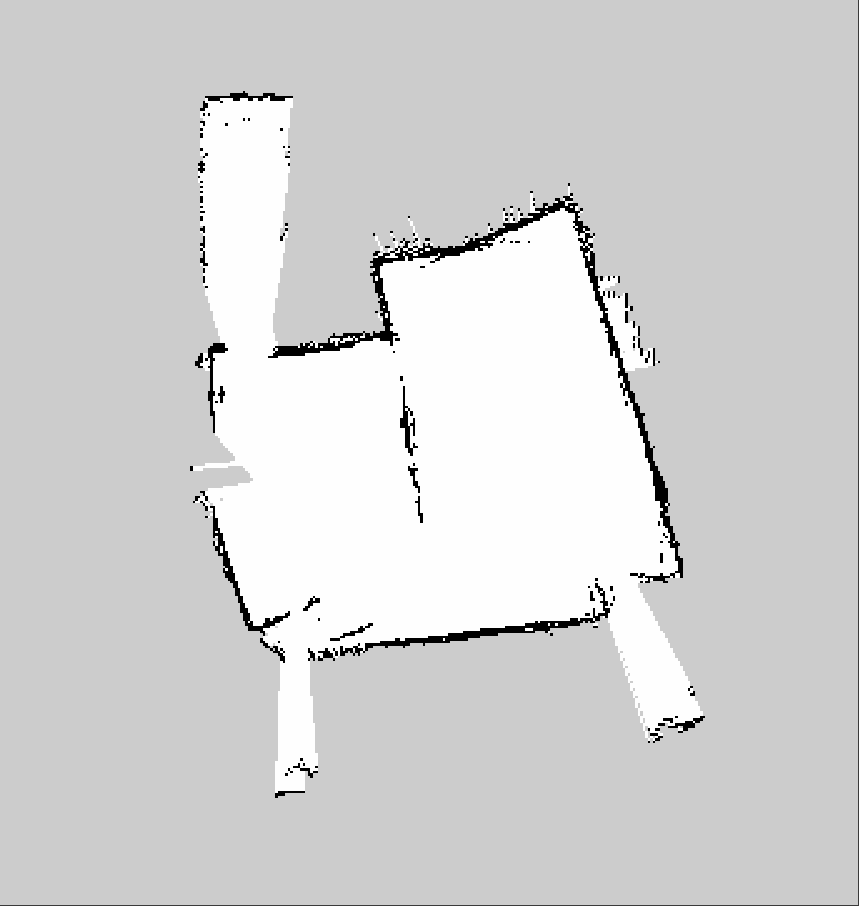
\includegraphics[width=0.3\textwidth]{scan1.png}}
  \subfloat[$0.3; 0.2; 3.0$]{
    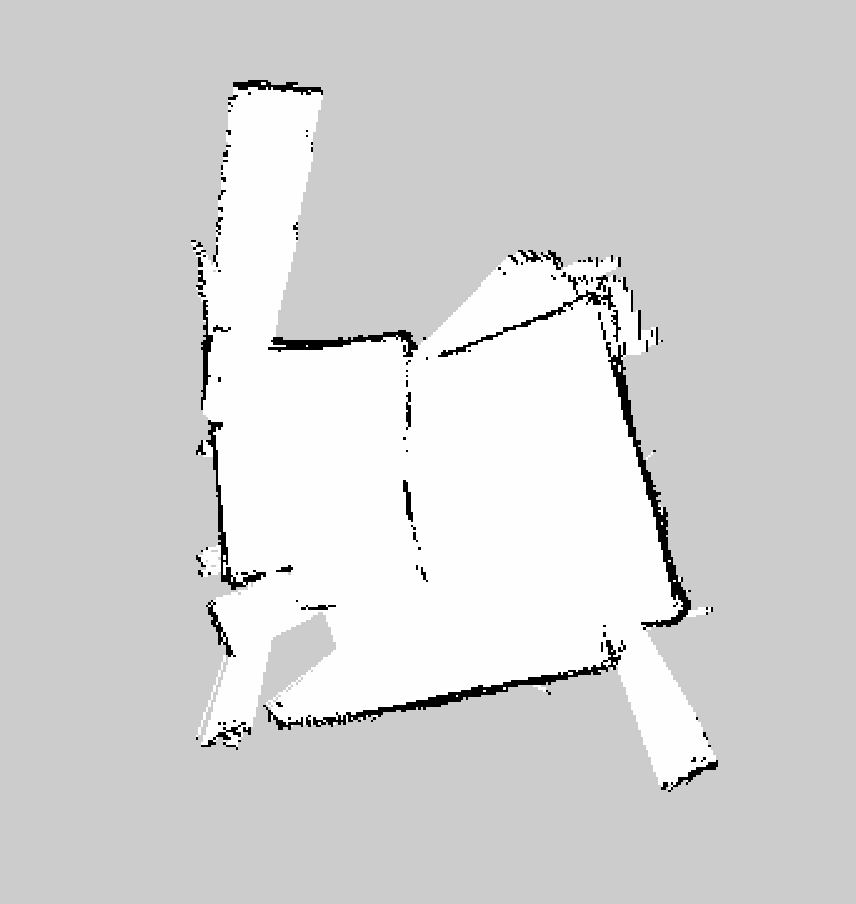
\includegraphics[width=0.3\textwidth]{scan2.png}}
  \subfloat[$0.5; 0.2; 3.0$]{
    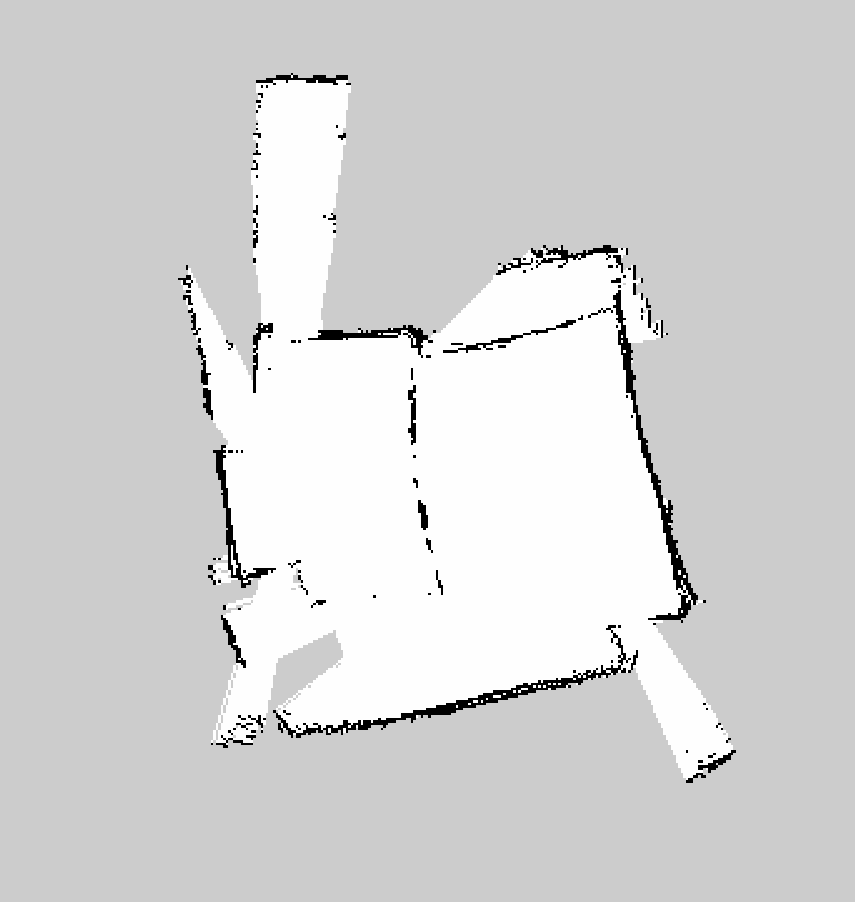
\includegraphics[width=0.3\textwidth]{scan3.png}}
 \caption{Resultados para diferentes parámetros de \texttt{linearUpdate}, \texttt{angularUpdate} y \texttt{temporalUpdate}, respectivamente}
 \label{fig:scans_params}
\end{figure}

Otro parámetro que se ha cambiado para obtener mejores resultados es la distancia máxima de profundidad, \texttt{range\_max}, del nodo \texttt{depthimage\_to\_laserscan} comentada en el apartado \ref{depthimage_section}. Este valor está por defecto a 10 metros. Sin embargo, debido a la existencia de amplias ventanas y puertas, el resultado se veía muy influenciado por las distancias alejadas captadas a través de estas. El valor que ha originado mejores resultados es 7 metros.\\

\begin{figure}[H]
 \centering
  \subfloat[\texttt{range\_max} a 7 metros]{
    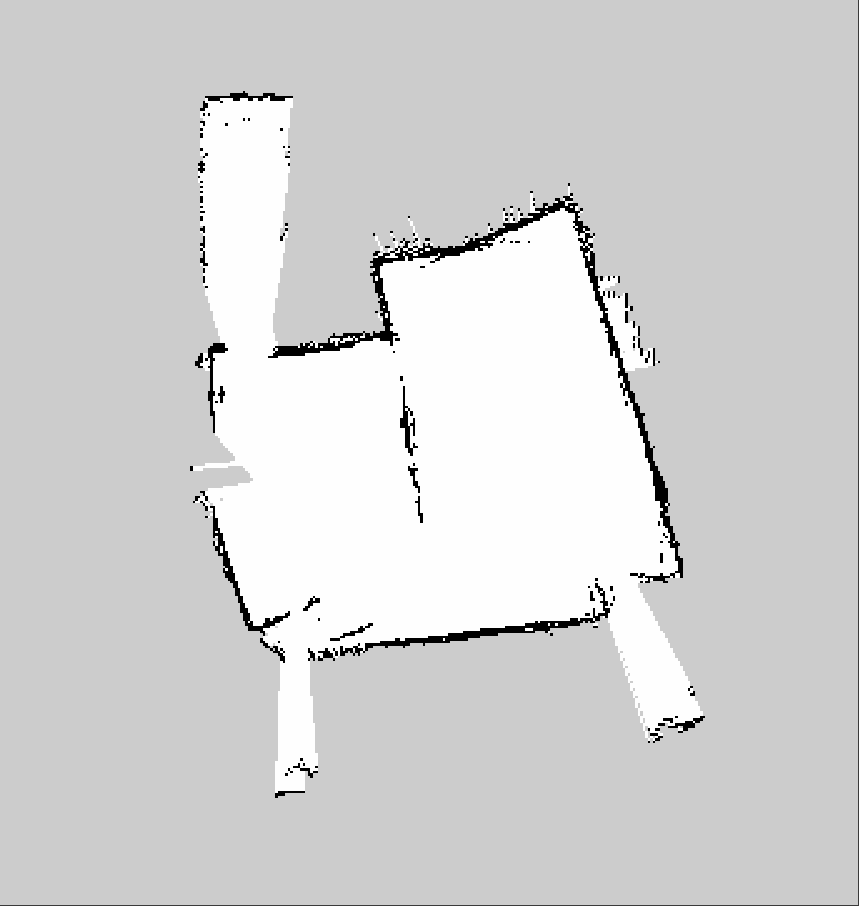
\includegraphics[width=0.4\textwidth]{scan1.png}}
  \subfloat[\texttt{range\_max} a 8 metros]{
    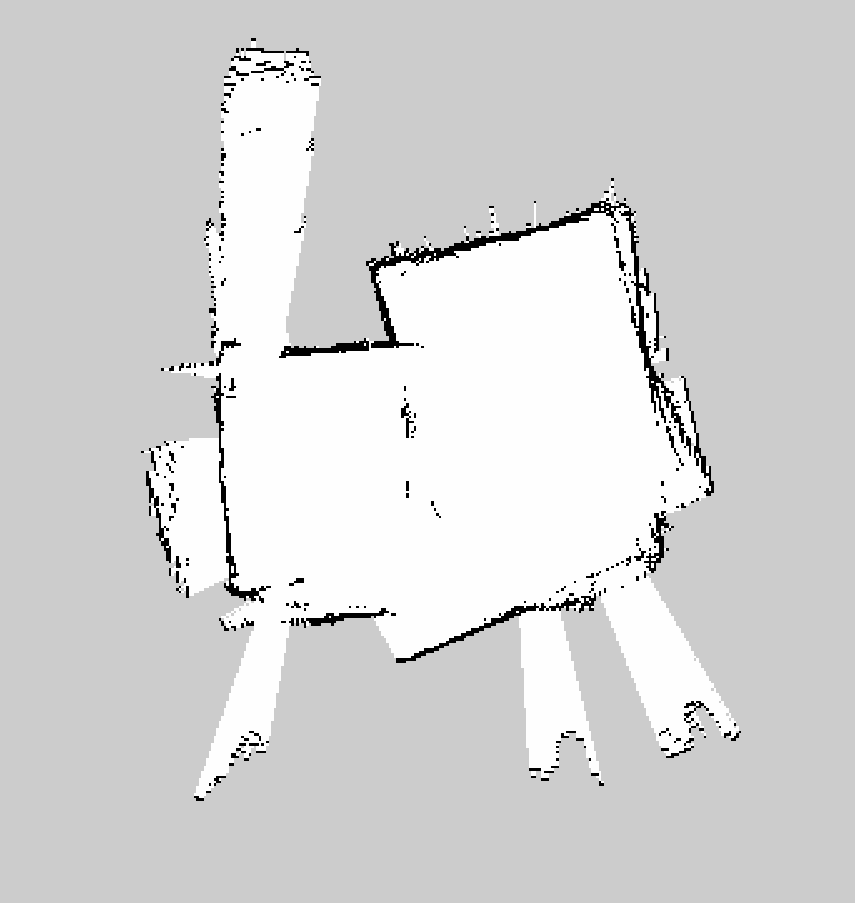
\includegraphics[width=0.4\textwidth]{scan4.png}}
 \caption{Resultados para distintos valores de distancia máxima. A mayor distancia máxima, mayor influencia de la información percibida por ventanas y puertas abiertas}
 \label{fig:scans_range}
\end{figure}


\section{Análisis de la fiabilidad de las detecciones}

YOLO es una de las redes neuronales más rápidas en el ámbito de la detección y localización de objetos en una imagen. Sin embargo, esta velocidad tan característica le hace sacrificar algo de exactitud en sus medidas, convirtiéndola en una red no del todo fiable. Aún así, continúa siendo de las mejores en este aspecto.\\

Con el nodo \texttt{write\_objects} obteníamos un archivo de texto con los datos en formato CSV, un formato que permite procesar los datos de manera sencilla. Este archivo contiene información sobre los objetos o clases detectadas, sus probabilidades, la pose del robot (posición y orientación) y el tiempo en el instante en que se detectaron dichos objetos. Para entender la trayectoria seguida por el robot, se propone la gráfica de la figura \ref{fig:graf_trayectoria}. Destacar que no comienza en el origen de coordenadas porque existre cierto desfase entre la ejecución de YOLO y los demás nodos, debido a la potencia necesaria para lanzarlo.\\

\begin{figure}[h]
	\begin{center} 
		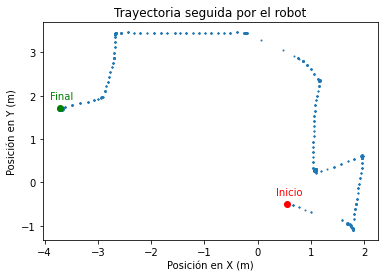
\includegraphics[width=0.6\textwidth]{graf_trayectoria.png}
	\end{center}
	\caption{Trayectoria seguida por el robot. El punto rojo indica el inicio de la trayectoria. El punto verde indica el final}
	\label{fig:graf_trayectoria}
\end{figure}

En la figura \ref{fig:graf_objetos} se muestra una gráfica de barras con el número de ocasiones que fueron detectadas cada una de las clases. Las clases `tvmonitor' (monitor de TV) y `chair' (silla) son las que más han sido detectadas, algo coherente con la distribución del laboratorio. La tercera clase más detectada ,`person' (persona), tampoco se escapa de la normalidad ya que durante la grabación había personas en el laboratorio. Las clases `mouse' (ratón) y `keyboard' (teclado), en principio, deberían haber sido tan frecuentes como las otras. Sin embargo, la cámara está prácticamente al mismo nivel que las mesas, lo que dificulta en gran medida el reconocimiento de estos objetos.\\

De todos los objetos que se han detectado, hay tres que no parecen pertenecer al entorno habitual de un laboratorio. Es el caso de `oven' (horno), `refrigerator' (frigorífico) y `microwave' (microondas). Este último es coherente ya que en el laboratorio hay uno y las detecciones las hace correctamente. Los otros son casos especiales que se explicarán a continuación.\\

\begin{figure}[h]
	\begin{center} 
		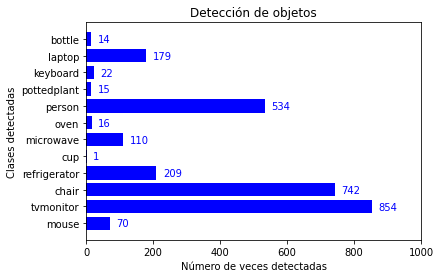
\includegraphics[width=0.7\textwidth]{graf_objetos.png}
	\end{center}
	\caption{Gráfica de objetos detectados. Muestra el número de veces que fue detectado cada uno de los objetos}
	\label{fig:graf_objetos}
\end{figure}

En este laboratorio no hay ningún horno, por lo que la detección de esta clase es errónea. Como se muestra en la figura \ref{fig:graf_oven}, `oven' solo se detecta en un momento durante la trayectoria. Revisando las imágenes del dataset, se puede ver lo que YOLO confunde con un horno, mostrado en la figura \ref{fig:det_oven}. Ciertamente, el objeto que detecta es muy parecido a los diales de control de un horno, por lo que es razonable la confusión.\\

\begin{figure}[h]
	\begin{center} 
		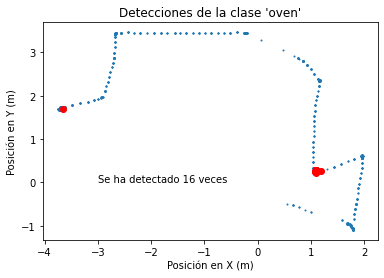
\includegraphics[width=0.6\textwidth]{graf_oven.png}
	\end{center}
	\caption{Momentos en los que se ha detectado la clase `oven'. Los puntos azules representan la trayectoria del robot, los rojos las veces que se detectó la clase}
	\label{fig:graf_oven}
\end{figure}

\begin{figure}[h]
	\begin{center} 
		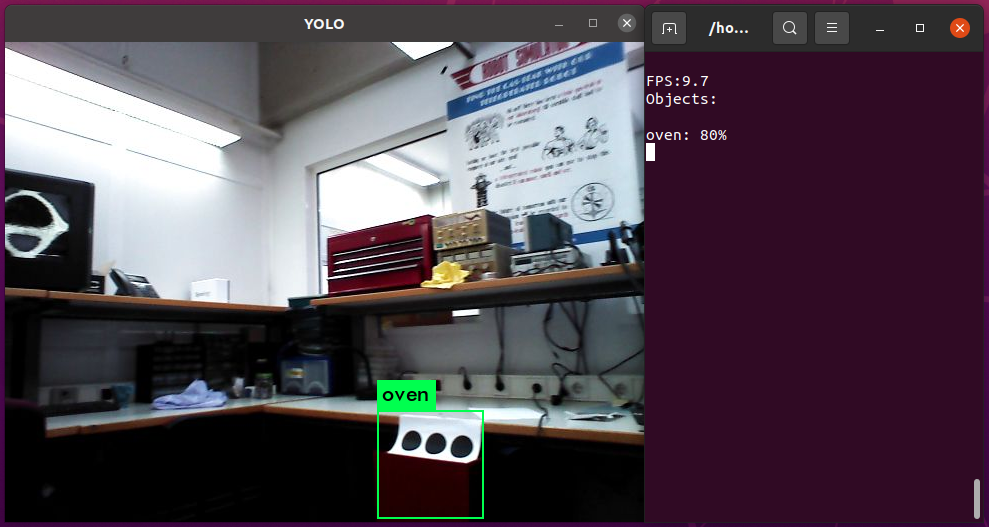
\includegraphics[width=0.8\textwidth]{oven.png}
	\end{center}
	\caption{Detección de la clase `oven' en la imagen}
	\label{fig:det_oven}
\end{figure}

En cambio, en el laboratorio sí que hay un frigorífico. Concretamente, un frigorífico compacto de una puerta. Sin embargo, pese a solamente haber uno, aparece en muchas ocasiones. Si obtenemos las posiciones en las que se detecta (figura \ref{fig:graf_refrigerator}), se puede ver como lo hace en posiciones muy distintas. Analizando las imágenes del dataset, se puede ver como, efectivamente, YOLO hace detecciones erróneas de la clase `refrigerator'. En la figura \ref{fig:det_refrigerator} se muestran dos detecciones erróneas y una correcta. Se puede ver como, en las detecciones incorrectas, los objetos detectados son similares a un frigorífico convencional.\\

\begin{figure}[h]
	\begin{center} 
		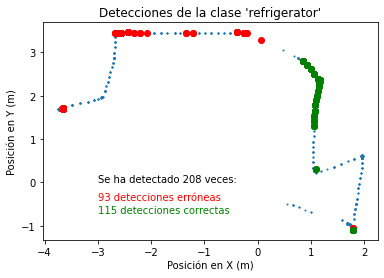
\includegraphics[width=0.6\textwidth]{graf_refrigerator.png}
	\end{center}
	\caption{Momentos en los que se ha detectado la clase `refrigerator'. Los puntos azules representan la trayectoria del robot, los rojos las veces que se detectó la clase}
	\label{fig:graf_refrigerator}
\end{figure}

\begin{figure}[H]
 \centering
  \subfloat[Detección errónea 1]{
    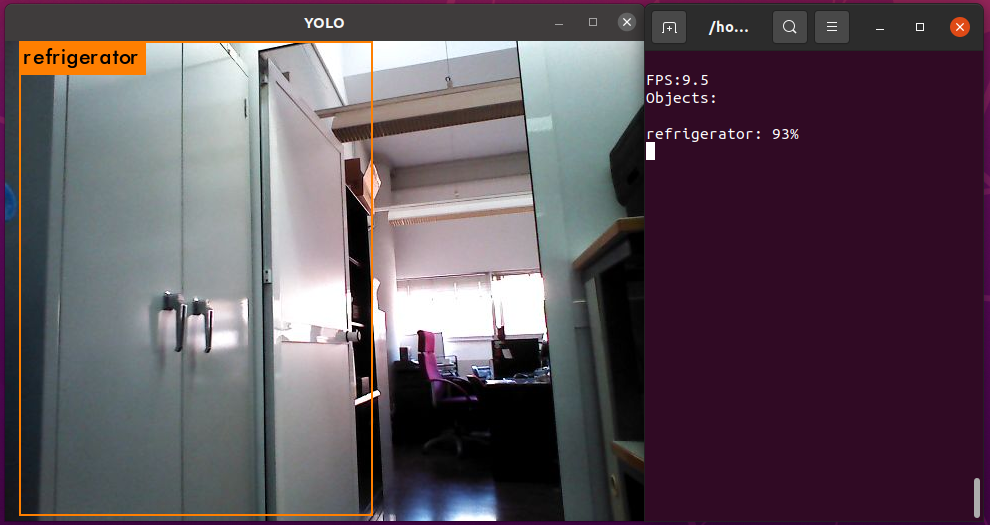
\includegraphics[width=0.45\textwidth]{refrigerator1.png}}
  \subfloat[Detección errónea 2]{
    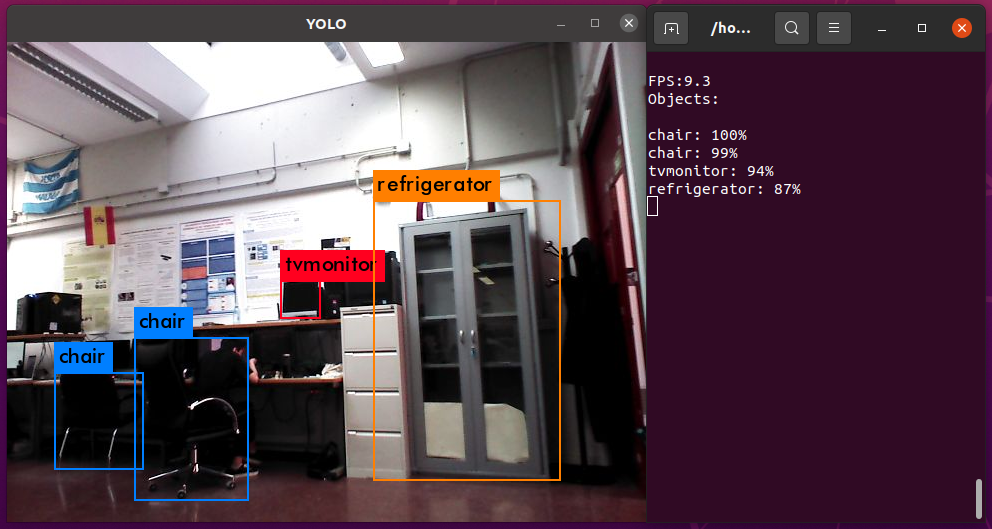
\includegraphics[width=0.45\textwidth]{refrigerator3.png}}
  \hspace{0.5cm}
  \subfloat[Detección correcta]{
    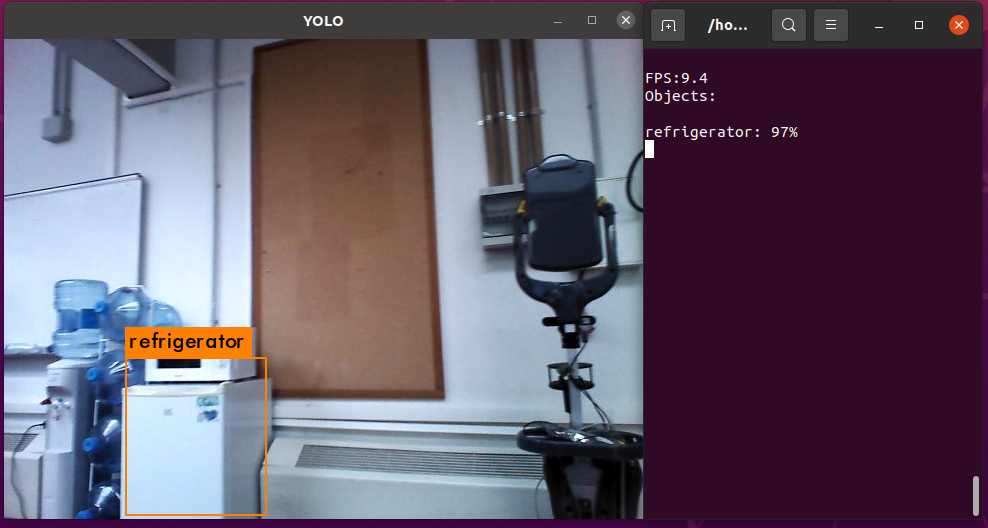
\includegraphics[width=0.6\textwidth]{refrigerator2.png}}
 \caption{Detecciones de la clase `refrigerator' en la imagen}
 \label{fig:det_refrigerator}
\end{figure}

\part{Conclusiones}

\chapter{Conclusiones, propuestas y líneas futuras}

En este capítulo se pretende, a partir de los resultados obtenidos y de todo el proceso llevado a cabo para conseguirlos, exponer las conclusiones a las que se han llegado. Además se expondrán algunas propuestas de cara a mejorar el procedimiento. Finalmente se trazarán posibles líneas de trabajo de cara al desarrollo futuro de este proyecto.\\

\section{Conclusiones}

Los láseres 2D son unos sensores que se caracterizan principalmente por su gran precisión y amplio campo de visión. Sin embargo, son elementos que encarecen en gran medida el presupuesto a dedicar para el diseño de un robot. Las cámaras RGBD, en cambio, son sensores muchos más asequibles, por lo que se deberían de tener en cuenta a la hora de generar \textit{floorplans} de la estructura del edificio o vivienda.\\

Como se ha mostrado en el capítulo \ref{chapter.resultados}, el resultado obtenido queda lejos lo ideal. El mapa obtenido mejora al láser en cuanto a la eliminación de los elementos no estructurales pero perjudica seriamente la rectitud de las líneas, provocando que el mapa pierda fiabilidad. Esto es debido a que los sensores RGBD son mucho menos precisos a la hora de calcular distancias, de ahí su gran diferencia de precio. Además, el dataset utilizado para comprobar el funcionamiento (el laboratorio de automática) no es el más amigable para este procedimiento debido a la gran cantidad de elementos que perjudican la medición a través de la cámara. Aún así, el resultado deja entrever que, con una correcta configuración y unas mejores condiciones del entorno, sería posible obtener un correcto floorplan estructural.\\

Por tanto, las conclusiones extraídas del desarrollo de este proyecto son las siguientes.

\begin{itemize}

	\item Las cámaras RGBD pueden llegar a ser un sustituto válido y asequible a la hora de generar floorplans que representen exclusivamente la estructura del edificio, sin elementos cambiantes como personas, muebles, etc.
	\item El entorno es el factor más determinante de cara a la efectividad del método. Un entorno con muchos elementos transparentes o con entrantes y salientes perjudican en gran medida los resultados obtenidos.
	\item La calibración de la cámara es muy importante si se quieren obtener resultados que puedan ser utilizados en la realidad.
	\item La comunidad de ROS es una de las más activas que se pueden encontrar. Existen miles de usuarios que aportan paquetes con funciones que abarcan prácticamente todos los ámbitos de la robótica. Por lo tanto, antes de comenzar a desarrollar alguna función, mejor comprobar si alguien ya lo ha hecho, algo que, vista la inmensitud de su comunidad, será lo más probable. Además, ROS cuenta con su propio foro donde compartir problemas y sus soluciones, ayudando en gran medida a usuarios novatos.
	\item La red neuronal YOLO, entrenada para la detección de objetos, pese a no ser del todo fiable, cumple su función. Sin embargo, muchos de los elementos del dataset no ha sido capaz de detectarlos, por lo que no hay que confiar completamente de sus mediciones.
	\item El manejo de datos con \textit{Python} y \textit{Pandas}
 resulta realmente sencillo. Complementándolo con la librería \textit{Matplotlib} se convierte en una poderosa herramienta para el análisis y la representación de los datos.
 	\item \textit{Linux}, pese a resultar inicialmente más complicado de comprender que otros sistemas operativos como \textit{Windows} o \textit{MacOS}, tiene numerosas características que lo convierten en una herramienta muy potente para el desarrollo, como la instalación por paquetes o el debugging.

\end{itemize}

\section{Propuestas y líneas futuras}

Hay aspectos de este trabajo que, una vez analizado de principio a fin, pudieran haberse hecho de otra forma y así, quizá, haber obtenido mejor resultado.\\

El dataset de datos (rosbag del laboratorio) no es el idóneo para esta tarea. Debido a todos sus entrantes y salientes y a las ventanas en la pared divisoria entre las dos estancias, el resultado obtenido no es del todo correcto. Lo mejor hubiera sido grabar al robot en un ambiente de vivienda convencional, con habitaciones, baños y cocinas. Además, la posición y orientación de la cámara no es la idónea. Dado que los elementos se encuentran mayoritariamente en la parte inferior de las paredes, lo ideal sería situar la cámara en una posición más alta que la del dataset, con una orientación paralela al plano del suelo.\\

YOLO utiliza una serie de pesos para detectar los objetos. Una interesante línea futura para este proyecto sería investigar los distintos datasets de pesos disponibles para YOLO y cuáles convendría utilizar en un entorno de laboratorio de ingenierías como con el que se ha trabajado.\\

Dado que el principal problema de los resultados obtenidos es la curvatura acaecida en las paredes medidas, sería conveniente buscar los parámetros que se ajustan concretamente a la cámara utilizada para generar el dataset. Posiblemente, una correcta configuración de los parámetros intrínsecos de la cámara, generará una mejoría en los resultados.\\


\part{Apéndices}

\appendix

\chapter{Otras herramientas utilizadas}

En este apéndice se expondrán las herramientas que se han utilizado para desarrollar el trabajo que no se explican en los capítulos anteriores pero que han sido necesarias poder alcanzar el objetivo. Principalmente se explicarán brevemente las librerías que se han utilizado en C++ y Python.\\

\section{Librerías y paquetes}

\subsection{\textit{message\_filters}}

Es un paquete de ROS que proporciona una serie de filtros capaces de recibir mensajes y enviarlos pasado un tiempo determinado en función de la necesidad dictaminada por el filtro. Está diseñado por Josh Faust, Vijay Pradeep y Dirk Thomas.\\

Para este proyecto se ha utilizado el filtro de sincronización o \textit{time synchronizer}. Este filtro se encarga de recibir mensajes de distintos topics y enviarlos sólo cuando se haya recibido un mensaje de cada uno de los topics con la misma marca temporal (\textit{timestamp)}. Concretamente se utiliza en el nodo \texttt{sync\_info}, para sincronizar los mensajes de la imagen de profundidad y de los parámetros de la cámara. \\ 

\subsection{\textit{fstream}}

Es una librería de C++ que permite la escritura en archivos. Se ha utilizado en el nodo \texttt{write\_objects} para escribir la información recibida de la pose y de la detección de objetos.\\

\subsection{\textit{libfreenect}}

\textit{libfreenect} es una librería que permite el acceso USB a la cámara Kinect de Microsoft. Es parte del proyecto \textit{OpenKinect}, una comunidad abierta que trabaja para implementar la posibilidad de uso de este dispositivo en todos los ordeanadores. Concretamente, se ha utilizado el paquete \texttt{freenect\_launch} que permite lanzar la cámara desde ROS.\\

Este paquete sirvió para tener una primera toma de contacto con los sensores RGBD, las imágenes de profundidad y las nubes de puntos.\\

\section{RVIZ}

RVIZ (ROS Visualization) es un visualizador 3D para ROS. Es un software que se instala junto con el framework. Su uso está prácticamente estandarizado en toda la comunidad de ROS.\\

Se utiliza para visualizar los mensajes que llegan a los topics. Permite visualizar poses, imágenes (en diferentes condificaciones),  mapas de ocupación, orientaciones, etc. e incluso permite incluir modelos 3D personalizados.\\

\section{Google Colab}

Colab, también conocido como ``Colaboratory'', es una herramienta creada por Google que permite a los usuarios programar y ejecutar código Python en el navegador, utilizando servicios alojados en la nube. Esta herramienta se ha utilizado para el análisis de los objetos detectados con la red neuronal. Las ventajas de utilizar esta plataforma son: no requiere configuración, da acceso gratuito a GPUs y permite compartir contenido fácilmente.\\

\section{CUDA: Compute Unified Device Architecture} \label{apendA.cuda}

CUDA es un conjunto de herramientas de desarrollo creadas por Nvidia que permiten a los programadores usar una variación del lenguaje de programación C (CUDA C) para coificar algoritmos GPU de Nvidia. Tiene como objetivo explitar las ventajas de las GPU frente a las CPU de propósito general utilizando el paralelismo que ofreccen sus múltiples núcleos, que permiten lanzar un altísimo número de procesos simultáneos \cite{cuda}.\\

Las principales ventajas de este sistema de computación son:

\begin{itemize}

	\item Lecturas dispersas. Se puede consultar cualquier posición en memoria.
	\item Memoria compartida. CUDA pone a disposición un área de memoria de entre 16KB y 48KB que se compartirá entre hilos del mismo bloque, pudiéndose utilizar como memoria caché.
	\item Lecturas más rápidas de y hacia la GPU.
	\item Soporte para enteros y operadores a nivel de bit.

\end{itemize}

\section{LaTex y TexMaker}

\LaTeX \, es un sistema de composición de textos, orientado a la creación de documentos escritos de alta calida tipográfica. Por sus característica, es ampliamente utilizado para la generación de documentos científicos. Este software se ha utilizado con la distro \textit{TexLive} y el software \textit{TexMaker} para la generación de este documento.\\

\section{Draw.io}

\textit{Draw.io} es un recurso web gratuito que sirve para realizar grafos. Todos los diagramas de este trabajo se han creado con esta herramienta. Se ha utilizado por su facilidad de uso y por la oportunidad de hacerlo online sin la obligación de instalar ningún software adicional.\\

\chapter{Código de los nodos diseñados}

\section{Nodo \texttt{cam\_info}}

\subsection*{\texttt{cam\_info.hpp}}

\lstset{style=cppstyle}
\vspace{0.2cm}
\lstinputlisting[language=C++, caption=Código del archivo \texttt{cam\_info.hpp}]{codes/cam_info.hpp}
\vspace{0.4cm}

\subsection*{\texttt{cam\_info.cpp}}

\vspace{0.2cm}
\lstinputlisting[language=C++, caption=Código del archivo \texttt{cam\_info.cpp}]{codes/cam_info.cpp}
\vspace{0.4cm}

\subsection*{\texttt{main\_cam\_info.cpp}}

\vspace{0.2cm}
\lstinputlisting[language=C++, caption=Código del archivo \texttt{main\_am\_info.cpp}]{codes/main_cam_info.cpp}
\vspace{0.4cm}

\section{Nodo \texttt{sync\_info}}

\lstset{style=pythonstyle}
\vspace{0.2cm}
\lstinputlisting[language=Python2, caption=Código del archivo \texttt{sync\_info.py}]{codes/sync_info.py}
\vspace{0.4cm}

\section{Nodo \texttt{write\_objects}}

\subsection*{\texttt{write\_objects.hpp}}

\lstset{style=cppstyle}
\vspace{0.2cm}
\lstinputlisting[language=C++, caption=Código del archivo \texttt{write\_objects.hpp}]{codes/write_objects.hpp}
\vspace{0.4cm}

\subsection*{\texttt{write\_objects.cpp}}

\vspace{0.2cm}
\lstinputlisting[language=C++, caption=Código del archivo \texttt{write\_objects.cpp}]{codes/write_objects.cpp}
\vspace{0.4cm}

\subsection*{\texttt{main\_write\_objects.cpp}}

\vspace{0.2cm}
\lstinputlisting[language=C++, caption=Código del archivo \texttt{main\_write\_objects.hpp}]{codes/main_write_objects.cpp}
\vspace{0.4cm}

\printbibliography


\end{document}